% !Mode:: "TeX:UTF-8"
% Translator: Yujun Li 
\chapter{\glsentrytext{ML}基础}
\label{chap:machine_learning_basics}
\gls{DL}是\gls{ML}的一个特定分支。
要想学好\gls{DL},必须对\gls{ML}的基本原理有深刻的理解。
本章将探讨贯穿本书其余部分的一些\gls{ML}重要原理。
我们建议新手读者或是希望更全面了解的读者参考一些更全面覆盖基础知识的\gls{ML}参考书,例如\cite{MurphyBook2012}或者\cite{bishop-book2006}。
如果你已经熟知\gls{ML},可以跳过前面的部分,前往第\ref{sec:challenges_motivating_deep_learning}节。
第\ref{sec:challenges_motivating_deep_learning}节涵盖了一些传统\gls{ML}技术的观点,这些技术对\gls{DL}的发展有着深远影响。

首先,我们将介绍学习算法的定义,并介绍一个简单的示例:\gls{linear_regression}算法。
接下来,我们会探讨拟合训练数据和寻找能够泛化到新数据的参数有哪些不同。
大部分\gls{ML}算法都设有\emph{超参数}(必须在学习算法外确定);我们将讨论如何使用额外的数据设置超参数。
\gls{ML}本质上属于应用统计学,更多关注于如何用计算机统计地估计复杂函数,不怎么关心这些函数的置信区间;因此我们会探讨两种统计学中主要的方法:频率估计和\gls{bayesian_inference}。
大部分\gls{ML}算法可以分成\gls{supervised_learning}和\gls{unsupervised_learning}两类;我们将探讨不同的分类,并为每类都介绍一些简单的\gls{ML}算法作为示例。
大部分\gls{DL}算法都基于\gls{SGD}求解。
我们将介绍如何组合不同的算法部分,例如优化算法、\gls{cost_function}、模型和\gls{dataset},来建立一个\gls{ML}算法。
最后在第\ref{sec:challenges_motivating_deep_learning}节,我们会介绍一些限制传统\gls{ML}泛化能力的因素。
为解决这些问题,这些挑战促进了\gls{DL}的发展。

% -- 95 --

\section{学习算法}
\label{sec:learning_algorithms}
\gls{ML}算法是一种可以从数据中学习的算法。
然而,我们所谓的``学习''是什么意思呢?
\cite{Mitchell:1997:ML}提供了一个简洁的定义:``对于某类任务$T$和\gls{performance_measures}$P$,一个计算机程序被认为可以从\gls{experience}$E$中学习是指,它的性能在任务$T$和性能测量$P$上通过\gls{experience}$E$有所提升。''
\gls{experience}$E$,任务$T$和性能测量$P$的定义范围非常宽广,在本书中我们并不会去试图解释这些定义的具体意义。
相反,我们会在接下来的章节中提供直观的解释和示例来介绍不同的任务、\gls{performance_measures}和\gls{experience},这些将被用来构建\gls{ML}算法。

\subsection{任务,$T$}
\label{sec:the_task_t}
\gls{ML}可以让我们应对一些由人来写和设计固定程序很难解决的问题。
从科学和哲学的角度来看,\gls{ML}受到关注是因为发展我们对\gls{ML}的认识需要发展我们对智能背后原理的理解。

如果考虑``任务''比较正式的定义,那么学习的过程并不是任务。
学习是我们所谓的获取完成任务的能力。
例如,我们的目标是会行走的机器人,那么行走便是任务。
我们可以编程让机器人学会如何行走,或者可以编写特定的指令,人工指导机器人如何行走。

通常\gls{ML}任务被定义为\gls{ML}系统该如何处理\firstgls{example:chap5}。
\gls{example:chap5}是指我们从某些希望\gls{ML}系统处理的对象或事件中收集到的已经量化的\firstgls{feature}的集合。
我们通常会将\gls{example:chap5}表示成一个向量$\Vx\in\SetR^n$,其中向量的每一个元素$x_i$是一个\gls{feature}。
例如,一张图片的\gls{feature}通常是指这张图片的像素。

% -- 96 --

\gls{ML}可以解决很多类型的任务。
\gls{ML}任务中一些非常常见任务列举如下:
\begin{itemize}
    \item \textbf{分类}:
    在这类任务中,计算机程序被要求指定某些输入属于$k$类中的哪一类。
    为了完成这个任务,学习算法通常被要求返回一个函数$f:\SetR^n \to \{1,\dots,k\}$。
    当$y=f(\Vx)$时,模型为向量$\Vx$所代表的输入指定数字码$y$所代表的类别。
    还有一些其他的分类问题,例如,$f$输出的是不同类别的概率分布。
    分类任务中有一类是对象识别,输入是图片(通常用一组像素亮度值表示),输出是表示图片物体的数字码。
    例如Willow Garage PR2机器人像服务员一样识别不同饮料,并送给下命令的顾客\citep{Goodfellow2010}。
    现代对象识别的最好工作是基于\gls{DL}的\citep{Krizhevsky-2012-small,Ioffe+Szegedy-2015}。
    对象识别同时也是计算机识别人脸的基本技术,可用于标记相片集中的人脸\citep{Taigman-et-al-CVPR2014},有助于计算机更自然地和用户交互。
    
    \item \textbf{输入缺失分类}:
    当输入向量的每个衡量不被保证的时候,分类问题将会更有挑战。
    为了解决分类任务,学习算法只需要定义\emph{一个}从输入向量映射到输出类别的函数。
    当一些输入可能丢失时,学习算法必须学习\emph{一组}函数,而不是单个分类函数。
    每个函数对应着分类具有不同缺失输入子集的$\Vx$。
    这种情况在医疗诊断中经常出现,因为很多类型的医学测试是昂贵的,对身体有害的。
    有效地定义这样一个大集合函数的方法是学习所有相关变量的概率分布,然后通过边缘化缺失变量来解决分类任务。 
    使用$n$个输入变量,我们现在可以获得每个可能的缺失输入集合所需的所有$2^n$个不同的分类函数,但是计算机程序仅需要学习一个描述联合概率分布的函数。
    参见\cite{Goodfellow-et-al-NIPS2013}了解以这种方式将深度概率模型应用于这样任务的示例。 
    本节中描述的许多其他任务也可以推广到缺失输入的情况; 缺失输入分类只是\gls{ML}可以做的一个示例。
    
% -- 97 --

    \item \textbf{回归}:这类任务中,计算机程序会给定输入预测数值。
    为了解决这个问题,学习算法会输出函数$f:\SetR^n \to \SetR$。
    除了返回结果的形式不一样外,这类问题和分类问题是很像的。
    这类任务的一个示例是预测投保人的索赔金额(用于设置保险费),或者预测证券未来的价格。
    这类预测也用在算法交易中。
    
    \item \textbf{\gls{transcribe}}:
    这类任务中,\gls{ML}系统观测一些相对非结构化表示的数据,并\gls{transcribe}信息为离散的文本形式。
    例如,光学字符识别要求计算机程序根据文本图片返回文字序列(ASCII码或者Unicode码)。
    谷歌街景使用\gls{DL}以这种方式处理街道编号\citep{Goodfellow+et+al-ICLR2014a}。
    另一个例子是语音识别,计算机程序输入一段音频波形,输出一序列音频记录中所说的字符或单词ID的编码。
    \gls{DL}是现代语音识别系统的重要组成部分,广泛用于各大公司,包括微软,IBM和谷歌\citep{Hinton-et-al-2012}。

    \item \textbf{机器翻译}:在机器翻译任务中,输入是一种语言的符号序列,计算机程序必须将其转化成另一种语言的符号序列。
    这通常适用于自然语言,如将英语译成法语。
    最近,\gls{DL}已经开始在这个任务上产生重要影响\citep{Sutskever-et-al-NIPS2014,Bahdanau-et-al-ICLR2015-small}。

    \item \textbf{结构化输出}:结构化输出任务涉及到输出是不同元素之间重要关系的向量(或者是含多个值的其他数据结构)的任务。
    这是一个很大的范畴,包括上面\gls{transcribe}任务和翻译任务在内的很多其他任务。
    例如语法分析---映射自然语言句子到语法结构数,并标记树的节点为动词,名词,副词等等。
    参考\cite{Collobert-AISTATS2011}应用\gls{DL}到语法分析。
    另一个例子是图像的像素级分割,将每一个像素分配到特定类别。
    例如,\gls{DL}可用于标注航拍照片中的道路位置\citep{MnihHinton2010}。
    在这些标注型的任务中,输出的结构形式不需要和输入尽可能相似。
    例如,在图片标题中,计算机程序观察到一幅图,输出描述这幅图的自然语言句子\citep{Kiros-et-al-ICML2014,Kiros-et-al-arxiv2014,Mao-et-al-2014,Vinyals-et-al-CVPR2015,Donahue-et-al-arxiv2014,Karpathy+Li-CVPR2015,Fang-et-al-CVPR2015,Xu-et-al-ICML2015}。
    这类任务被称为\emph{结构化输出任务}是因为输出值之间内部紧密相关。
    例如,图片标题程序输出的单词必须组合成一条通顺的句子。

% -- 98 --

    \item \textbf{异常检测}:这类任务中,计算机程序从一组事件或物体中筛选并标记不正常或非典型的个体。
    异常检测任务的一个例子是信用卡欺诈检测。
    通过对你的购买习惯建模,信用卡公司可以检测到你的卡是否被滥用。
    如果窃贼窃取你的信用卡或信用卡信息,窃贼采购物品的分布通常和你的不同。
    当该卡发生了不正常的购买行为时,信用卡公司可以尽快冻结该卡以防欺诈。
    参考\cite{chandola2009anomaly}了解欺诈检测方法。

    \item \textbf{合成和采样}:这类任务中,\gls{ML}程序生成一些和训练数据相似的新\gls{example:chap5}。
    通过\gls{ML},合成和采样可能在媒体应用中非常有用,可以避免艺术家大量昂贵或者乏味的手动工作。
    例如,视频游戏可以自动生成大型物体或风景的纹理,而不是让艺术家手动标记每个像素\citep{Luo+al-AISTATS2013-small}。
    在某些情况下,我们希望采样或合成过程可以根据给定的输入来生成一些特定类型的输出。
    例如,在语音合成任务中,我们提供书写的句子,要求程序输出这个句子语音的音频波形。
    这是一类\emph{结构化输出任务},但是多了每个输入并非只有一个正确输出的条件,我们明确希望输出有很大的偏差,使结果看上去更加自然和真实。

    \item \textbf{缺失值归责}:这类任务中,\gls{ML}算法给定一个新\gls{example:chap5}$\Vx\in\SetR^n$,$\Vx$中某些元素$x_i$缺失。
    算法必须预测这些缺失值。

% -- 99 --

    \item \textbf{降噪}:这类任务中,\gls{ML}算法的输入是,由未知破坏过程从\emph{干净\gls{example:chap5}}$\Vx \in \SetR^n$得到的\emph{污染\gls{example:chap5}}$\tilde{\Vx} \in \SetR^n$。
    算法根据污染后的\gls{example:chap5}$\tilde{\Vx}$预测干净的\gls{example:chap5}$\Vx$,或者更一般地预测条件概率分布$P(\Vx|\tilde{\Vx})$。
    
    \item \textbf{密度估计}\textbf{或}\textbf{概率质量函数估计}:在密度估计问题中,\gls{ML}算法学习函数$p_{\text{model}}:\SetR^n \to \SetR$,其中$p_{\text{model}}(\Vx)$可以解释成\gls{example:chap5}采样空间的概率密度函数(如果$\RVx$是连续的)或者概率质量函数(如果$\RVx$是离散的)。
    要做好这样的任务(当我们讨论\gls{performance_measures}$P$时,我们会明确定义任务是什么),算法需要学习它观测到的数据的结构。
    算法必须知道什么情况\gls{example:chap5}聚堆出现,哪些情况不太可能出现。
    以上描述的大多数任务都要求学习算法至少能隐式地抓住概率分布的结构。
    密度分布可以让我们显式地抓住该分布。
    原则上,我们可以在该分布上计算以便解决其他任务。
    例如,如果我们通过密度估计得到了概率分布$p(\Vx)$,我们可以用该分布解决输入缺失问题。
    如果$x_i$的值是缺失的,但是其他的变量值$\Vx_{-i}$已知,那么我们可以得到条件概率分布$p(x_i|\Vx_{-i})$。
    现实中,密度估计并非能够解决所有这类问题,因为在很多情况下$p(\Vx)$是难以计算的。
\end{itemize}

当然,还有很多其他或其他类型的任务。
这里我们列举的任务类型只是用来介绍\gls{ML}可以做哪些任务,并非对\gls{ML}能够做的任务进行刚性分类。

\subsection{\glsentrytext{performance_measures},$P$}
\label{sec:the_performance_measure_p}
为了评估\gls{ML}算法的能力,我们必须设计其性能的定量衡量。
通常\gls{performance_measures}$P$是对系统执行的任务$T$特定而言的。

对于诸如分类,缺失输入分类,和\gls{transcribe}任务,我们通常衡量模型的\firstgls{accuracy}。
\gls{accuracy}是指该模型输出正确结果的\gls{example:chap5}比例。
我们也可以通过\firstgls{error_rate}得到相同的信息。
\gls{error_rate}是指该模型输出错误结果的\gls{example:chap5}比例。
我们通常把错误率称作$0-1$损失的期望。
在一个特定的\gls{example:chap5}上,如果结果是对的,那么$0-1$损失是$0$;否则是$1$。
对于密度估计这类任务而言,衡量准确率,错误率或者其他类型的$0-1$损失是没有意义的。
反之,我们必须使用不同的性能指标,使该模型对每个\gls{example:chap5}都输出一个连续数值的得分。
最常用的方法是输出模型在一些\gls{example:chap5}上概率对数的平均值。


% -- 100 --

通常,我们比较感兴趣\gls{ML}算法在未观测数据上的性能如何,因为这将决定它在现实生活中的性能如何。
因此,我们从训练\gls{ML}系统的训练集数据中用一部分作为\firstgls{test_set}数据评估系统性能。
\gls{performance_measures}的选择或许看上去简单且客观,但是选择一个与系统理想表现对应的\gls{performance_measures}通常是很难的。

在某些情况下,这是因为很难决定应该衡量什么。
例如,在执行\gls{transcribe}任务时,我们是应该衡量系统\gls{transcribe}整个序列的准确率,还是应该用一个更细粒度的指标,对序列中部分正确的元素给以正面评价?
在执行回归任务时,我们应该惩罚频繁犯一些中等错误的系统多一点,还是较少犯错但是犯很大错误的系统多一点?
这些设计的选择取决于应用。

还有一些情况,我们知道应该衡量哪些数值,但是衡量它们难度不太现实。
例如,这频繁出现在密度估计中。
很多最好的模型都是隐式地表示概率分布。
在许多这类模型中,计算空间中特定点的真实概率是不可行的。
在这些情况下,我们必须设计一个仍然对应于设计对象的替代标准,或者设计一个理想标准的良好近似。

\subsection{\glsentrytext{experience},$E$}
\label{sec:the_experience_e}
根据学习过程中的不同\gls{experience},\gls{ML}算法可以大致分类为\firstgls{unsupervised}和\firstgls{supervised}。

本书中的大部分学习算法可以理解成在整个\firstgls{dataset}上获取\gls{experience}。
\gls{dataset}是指很多\gls{example:chap5}组成的集合,如第5.1.1节的定义。有时我们也将\gls{example:chap5}称为\firstgls{data_points}。

% -- 101 --

统计学家和\gls{ML}研究者使用很久的\gls{dataset}之一是Iris(鸢尾花卉)\gls{dataset}\citep{Fisher-1936}。
它是$150$个鸢尾花卉植物不同部分测量结果的集合。
每个单独的植物对应一个\gls{example:chap5}。
每个\gls{example:chap5}的\gls{feature}是该植物不同部分的测量结果:萼片长度,萼片宽度,花瓣长度和花瓣宽度。
该\gls{dataset}还记录每个植物属于什么品种。
这个\gls{dataset}展示了三个不同的物种。

\firstgls{unsuper_learn_algo}训练含有很多\gls{feature}的\gls{dataset},然后学习出这个\gls{dataset}上有用的结构性质。
在\gls{DL}中,我们通常要学习生成\gls{dataset}的整个概率分布,显式地,比如密度估计,或是隐式地,比如合成或降噪。
还有些其他的\gls{unsupervised_learning}算法会执行其他的任务,例如聚类,将\gls{dataset}分成相似\gls{example:chap5}的集合。

\firstgls{super_learn_algo}训练含有很多\gls{feature}的\gls{dataset},不过\gls{dataset}中的\gls{example:chap5}都有一个\firstgls{label}或\firstgls{target}。
例如,Iris\gls{dataset}注明了每个鸢尾花卉\gls{example:chap5}属于什么品种。
\gls{supervised_learning}算法通过研究Iris\gls{dataset},学习如何根据测量结果将\gls{example:chap5}划分到三个不同品种。

大致说来,\gls{unsupervised_learning}涉及到观察随机向量$\RVx$的好几个\gls{example:chap5},试图隐式或显式地学习出概率分布$p(\RVx)$,或者是该分布一些有意思的性质;
而\gls{supervised_learning}包含观察随机向量$\RVx$及其相关联的值或向量$\RVy$,然后从$\RVx$预测$\RVy$,通常是估计$p(\RVy|\RVx)$。
术语\firstgls{supervised}源自这样一个视角,教员或者老师提供\gls{target}$\RVy$给\gls{ML}系统,指导其应该做什么。
在\gls{unsupervised_learning}中,没有教员或者老师,算法必须学会在没有指导的情况下让数据有意义。

\gls{unsupervised_learning}和\gls{supervised_learning}不是严格定义的术语。
它们之间界线通常是模糊的。
大部分\gls{ML}技术可以用于这两个任务。
例如,概率的链式法则表明对于向量$\RVx\in\SetR^n$,联合分布可以分解成
\begin{equation}
    p(\RVx) = \prod_{i=1}^n p(\RSx_i \mid \RSx_1,\dots,\RSx_{i-1}) .
\end{equation}
该分解意味着我们通过将其拆分成$n$个\gls{unsupervised_learning},来解决表面上的\gls{unsupervised_learning}$p(\Vx)$。
另外,我们求解\gls{supervised_learning}问题$p(y|\RVx)$时,也可以使用传统的\gls{unsupervised_learning}技巧学习联合分布$p(\RVx,y)$,然后推测
\begin{equation}
    p(y|\RVx) = \frac{p(\RVx,y)}{\sum_{y'}p(\RVx,y')}.
\end{equation}
尽管\gls{unsupervised_learning}和\gls{supervised_learning}并非完全正式或不同的概念,它们确实有助于粗略分类我们研究\gls{ML}算法时遇到的问题。
传统地,人们将回归,分类,或者结构化输出问题称为\gls{supervised_learning}。
支持其他任务的密度估计通常被称为\gls{unsupervised_learning}。

% -- 102 --

学习范式的其他变种也是有可能的。
例如,半监督学习中,一些\gls{example:chap5}有监督\gls{target},但其他的没有。
在多实例学习中,\gls{example:chap5}的整个集合被标记为含有或者不含有该类的\gls{example:chap5},但是集合中单独的样本是没有标记的。
参考\cite{Kotzias2015}了解最近深度模型进行多实例学习的样例。

有些\gls{ML}算法并不是训练于一个固定的\gls{dataset}上。
例如,\firstgls{reinforcement_learning}算法会和环境进行交互,所以学习系统和它的训练过程会有反馈回路。
这类算法超出了本书的范畴。
请参考\cite{Sutton+Barto-98}或\cite{Bertsekas+Tsitsiklis-book1996}了解强化学习相关知识,\cite{Mnih2013}介绍了强化学习方向的\gls{DL}方法。

大部分\gls{ML}算法简单地训练于一个\gls{dataset}。
\gls{dataset}可以用很多不同方式来表示。
在所有的情况下,\gls{dataset}都是\gls{example:chap5}的集合,而\gls{example:chap5}是\gls{feature}的集合。

表示\gls{dataset}的常用方法是\firstgls{design_matrix}。
\gls{design_matrix}的每一行包含一个不同的\gls{example:chap5}。
每一列对应不同的\gls{feature}。
例如,Iris\gls{dataset}包含$150$个\gls{example:chap5},每个\gls{example:chap5}有4个\gls{feature}。
这意味着我们将该\gls{dataset}表示成\gls{design_matrix}$\MX\in\SetR^{150\times 4}$,其中$\MX_{i,1}$表示第$i$个植物的萼片长度,$\MX_{i,2}$表示第$i$个植物的萼片宽度,等等。
我们在本书中描述的大部分学习算法都是讲述它们是如何运行在\gls{design_matrix}\gls{dataset}上的。

当然,将一个\gls{dataset}表示成\gls{design_matrix},必须是可以将每一个\gls{example:chap5}表示成向量,并且这些向量的大小相同。
这一点并非永远可能。
例如,你有不同宽度和高度的照片的集合,那么不同的照片将会包含不同数量的像素。
因此不是所有的照片都可以表示成相同长度的向量。
第9.7节和第\ref{chap:sequence_modeling_recurrent_and_recursive_nets}章将会介绍如何处理这类异质问题的不同类型。
在上述的这类情况下,我们不会将\gls{dataset}表示成$m$行的矩阵,而是表示成$m$个元素的结合:$\{\Vx^{(1)},\Vx^{(2)},\dots,\Vx^{(m)}\}$。
这种表示方式并非意味着\gls{example:chap5}向量$\Vx^{(i)}$和$\Vy^{(j)}$有相同的大小。

% -- 103 --

在\gls{supervised_learning}中,\gls{example:chap5}包含一个\gls{label}或\gls{target}和一组\gls{feature}。
例如,我们希望使用学习算法从照片中识别物体。
我们需要明确哪些物体会出现在每张照片中。
我们或许会用数字编码表示,如$0$表示人,$1$表示车,$2$表示猫,等等。
通常当工作在包含观测\gls{feature}的\gls{design_matrix}$\MX$的\gls{dataset}时,我们也会提供一个\gls{label}向量$\Vy$,其中$y_i$表示\gls{example:chap5}$i$的\gls{label}。

当然,有时\gls{label}可能不止一个数。
例如,如果我们想要训练语音模型\gls{transcribe}整个句子,那么每个句子\gls{example:chap5}的\gls{label}是一个单词序列。

正如\gls{supervised_learning}和\gls{unsupervised_learning}没有正式的定义,\gls{dataset}或者\gls{experience}也没有严格的分类。
这里介绍的结构涵盖了大多数情况,但始终有可能为新的应用设计出新的结构。

\subsection{实例:\glsentrytext{linear_regression}}
\label{sec:example_linear_regression}
我们将\gls{ML}算法定义为通过某些任务上训练来提高计算机程序性能的算法,这种定义有点抽象。
为了使这个定义更具体点,我们展示一个简单的\gls{ML}实例:\firstgls{linear_regression}。
当我们介绍更多有助于理解\gls{ML}特性的概念时,我们会反复回顾这个实例。

顾名思义,\gls{linear_regression}解决回归问题。
换言之,我们的目标是建立一个系统,将向量$\Vx\in\SetR^n$作为输入,预测标量$y\in\SetR$作为输出。
\gls{linear_regression}的输出是其输入的线性函数。
让$\hat{y}$表示模型预测$y$应该取的值。
我们定义输出为
\begin{equation}
    \hat{y} = \Vw^\Tsp \Vx ,
\end{equation}
其中$\Vw\in\SetR^n$是\firstgls{parameters}向量。

\gls{parameters}是控制系统行为的值。
在这种情况下,$w_i$是系数,会和\gls{feature}$x_i$相乘之后全部加起来。
我们可以将$\Vw$看作是一组决定每个\gls{feature}如何影响预测的\firstgls{weights}。
如果\gls{feature}$x_i$对应的权重$w_i$是正的,那么\gls{feature}值增加,我们的预测值$\hat{y}$也会增加。
如果\gls{feature}$x_i$对应的权重$w_i$是负的,那么\gls{feature}值减少,我们的预测值$\hat{y}$也会减少。
如果\gls{feature}权重的大小很大,那么它对预测有很大的影响;如果\gls{feature}权重的大小是零,那么它对预测没有影响。

% -- 104 --

因此,我们可以定义任务$T$:通过输出$\hat{y} = \Vw^\Tsp \Vx$从$\Vx$预测$y$。
接下来我们需要定义\gls{performance_measures},$P$。

假设我们有$m$个输入\gls{example:chap5}组成的\gls{design_matrix},我们不用它来训练模型,而是评估模型性能如何。
我们也有每个\gls{example:chap5}对应的正确值$y$组成的回归\gls{target}向量。
因为这个\gls{dataset}只是用来评估性能,我们称之为\gls{test_set}。
我们将输入的\gls{design_matrix}记作$\MX^{\text(test)}$,回归\gls{target}向量记作$\Vy^{(\text{test})}$。

衡量模型性能的一种方法是计算模型在\gls{test_set}上的\firstgls{mean_squared_error}。
如果$\hat{\Vy}^{(\text{test})}$表示模型在\gls{test_set}上的预测值,那么\gls{mean_squared_error}表示为:
\begin{equation}
    \text{MSE}_{\text{test}} = \frac{1}{m} \sum_i ( \hat{\Vy}^{(\text{test})} - \Vy^{(\text{test})})_i^2.
\end{equation}
直观上,当$\hat{\Vy}^{(\text{test})} = \Vy^{(\text{test})}$时,我们会发现误差降为$0$。
我们也可以表示为
\begin{equation}
    \text{MSE}_{\text{test}} = \frac{1}{m} \norm{ \hat{\Vy}^{(\text{test})} - \Vy^{(\text{test})}}_2^2,
\end{equation}
所以当预测值和\gls{target}值之间的欧几里得距离增加时,误差也会增加。

为了得到一个\gls{ML}算法,我们需要设计一个算法,通过观察训练集$(\MX^{(\text{train})},\Vy^{(\text{train})})$是算法获得\gls{experience},以减少$\text{MSE}_{\text{test}}$的方式改进权重$\Vw$。
这样做的一种直观的方式(我们将在后续的第5.5.1节说明其合法性)是最小化训练集上的\gls{mean_squared_error},$\text{MSE}_{\text{train}}$。

最小化$\text{MSE}_{\text{train}}$,我们可以简单地求解它的导数为$\mathbf{0}$的情况:
\begin{equation}
\nabla_{\Vw} \text{MSE}_{\text{train}} = 0
\end{equation}
\begin{equation}
\Rightarrow \nabla_{\Vw} \frac{1}{m} \norm{ \hat{\Vy}^{(\text{train})} - \Vy^{(\text{train})}}_2^2 = 0
\end{equation}
\begin{equation}
\Rightarrow \frac{1}{m} \nabla_{\Vw} \norm{ \MX^{(\text{train})}\Vw - \Vy^{(\text{train})}}_2^2 = 0
\end{equation}
\begin{equation}
\Rightarrow \nabla_{\Vw} \left( \MX^{(\text{train})}\Vw - \Vy^{(\text{train})} \right)^\Tsp \left( \MX^{(\text{train})}\Vw - \Vy^{(\text{train})} \right) = 0
\end{equation}
\begin{equation}
\Rightarrow \nabla_{\Vw} \left( 
    \Vw^\Tsp \MX^{(\text{train})\Tsp}\MX^{(\text{train})}\Vw - 2\Vw^\Tsp\MX^{(\text{train})\Tsp} \Vy^{(\text{train})} + \Vy^{(\text{train})\Tsp}\Vy^{(\text{train})}  
  \right) = 0
\end{equation}
\begin{equation}
    \Rightarrow 2\MX^{(\text{train})\Tsp}\MX^{(\text{train})} \Vw  -
    2\MX^{(\text{train})\Tsp} \Vy^{(\text{train})}  = 0
\end{equation}
\begin{equation}
\label{eq:5.12}
    \Rightarrow \Vw =  \left(\MX^{(\text{train})\Tsp}\MX^{(\text{train})}
     \right)^{-1} \MX^{(\text{train})\Tsp} \Vy^{(\text{train})}
\end{equation}

% -- 105 --

通过式\ref{eq:5.12}给出解的系统方程被称为\firstgls{normal_equations}。
计算式\ref{eq:5.12}构成了一个简单的机器学习算法。
参考图\ref{fig:chap5_linreg}\gls{linear_regression}算法的动态示例。

\begin{figure}[!htb]
\ifOpenSource
\centerline{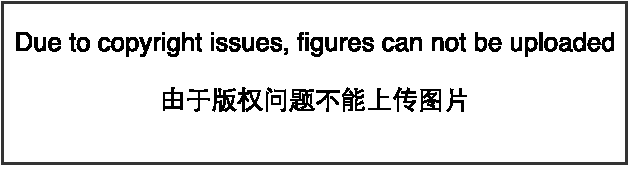
\includegraphics{figure.pdf}}
\else
\centerline{\includegraphics{Chapter5/figures/linreg_color}}
\fi
\caption{TODO}
\label{fig:chap5_linreg}
\end{figure}

值得注意的是,术语{\gls{linear_regression}}通常用来指稍微复杂一些,附加额外参数(截距项$b$)的模型。
在这个模型中,
\begin{equation}
    \hat{y} = \Vw^\Tsp \Vx + b,
\end{equation}
因此从参数到预测的映射仍是一个线性函数,而从\gls{feature}到预测的映射是一个仿射函数。
如此扩展到仿射函数意味着模型预测的曲线仍然看起来像是一条直线,只是这条直线没必要经过原点。
不通过添加偏置参数$b$,我们仍然可以使用仅含权重的模型,但是$\Vx$需要增加一项永远为$1$的元素。
对应于额外$1$的权重起到了偏置参数的作用。
当我们在本书中提到仿射函数时,我们会频繁地使用术语“线性”。

% -- 106 --

截距项$b$通常被称为仿射变换的\firstgls{bias_aff}参数。
这个术语的命名源自该变换的输出在没有任何输入时会偏移$b$。
它和统计偏差中指代统计估计算法的某个量的期望估计偏离真实值的意思是不一样的。

\gls{linear_regression}当然是一个极其简单且有局限的学习算法,但是它提供了一个说明学习算法如何工作的例子。
在接下来的小节中,我们将会介绍一些设计学习算法的基本原则,并说明如何使用这些原则来构建更复杂的学习算法。

\section{\glsentrytext{capacity},\glsentrytext{overfitting}和\glsentrytext{underfitting}}
\label{sec:capacity_overfitting_and_underfitting}
\gls{ML}的主要挑战是我们模型必须能够在先前未观测的新输入上表现良好,而不是只在训练集上效果好。
在先前未观测到的输入上表现良好的能力被称为\firstgls{generalization}。

通常情况下,当我们训练\gls{ML}模型时,我们可以访问训练集,在训练集上计算一些误差,被称之为\firstgls{training_error},并且我们会降低训练误差。
目前为止,我们讨论的是一个简单的优化问题。
\gls{ML}和优化不同的地方在于,我们也希望\firstgls{generalization_error},也被称为\firstgls{test_error},很低。
泛化误差被定义为新输入上误差的期望。
这里,期望取值自我们期望系统在现实中从输入分布中采样得到的不同可能值。

通常,通过评估衡量模型在从训练集分出来的\firstgls{test_set}\gls{example:chap5}上的性能,我们评估\gls{ML}模型的泛化误差。

在我们的\gls{linear_regression}实例中,我们通过最小化\gls{training_error}来训练模型,
\begin{equation}
    \frac{1}{m^{(\text{train})}} \norm{\MX^{(\text{train})}\Vw - \Vy^{(\text{train})}}_2^2,
\end{equation}
但是我们真正关心的是\gls{test_error},$\frac{1}{m^{(\text{test})}} \norm{\MX^{(\text{test})}\Vw - \Vy^{(\text{test})}}_2^2$。

% -- 107 --

当我们只能观测到训练集时,我们如何才能影响\gls{test_set}的性能呢?
\firstgls{SLT}提供了一些答案。
如果训练集和\gls{test_set}的数据是任意收集的,那么我们能够做的确实很有限。
如果我们可以对\gls{training_set}和\gls{test_set}数据的收集方式有些假设,那么我们能够对算法做些改进。

\gls{training_set}和\gls{test_set}数据通过\gls{dataset}上被称为\firstgls{DGP}的概率分布生成。
通常,我们会做一系列假设,被统称为\firstgls{iid}。
该假设是说,每个\gls{dataset}中的\gls{example:chap5}都是彼此\firstgls{independent},并且\gls{training_set}和\gls{test_set}是\firstgls{id},其上数据采样自相同的分布。
这个假设使我们能够在单个示例上用概率分布描述数据生成过程。
然后相同的分布可以被用来生成每一个训练\gls{example:chap5}和每一个测试\gls{example:chap5}。
我们将这个共享的潜在分布称为\firstgls{DGD},记作$p_{\text{data}}$。
这个概率框架和独立同分布假设允许我们数学地研究\gls{training_error}和\gls{test_error}之间的关系。

我们能观察到\gls{training_error}和\gls{test_error}之间的直接联系是,随机模型\gls{training_error}的期望和该模型\gls{test_error}的期望是一样的。
假设我们有概率分布$p(\Vx,y)$,从中重复采样生成\gls{training_set}和\gls{test_set}。
对于某个固定的$\Vw$,\gls{training_set}误差的期望恰好和\gls{test_set}误差的期望一样,这是因为这两个期望的计算都是用相同的数据集生成过程。
这两种情况的唯一区别是\gls{dataset}的名字不同。

当然,当我们使用\gls{ML}算法时,我们不会提前固定参数,然后从\gls{dataset}中采样。
我们会在训练集上采样,然后挑选参数去降低训练集误差,然后再在\gls{test_set}上采样。
在这个过程中,测试误差期望会大于或等于训练误差期望。
以下是决定\gls{ML}算法效果是否好的因素:
\begin{enumerate}
    \item 降低训练误差
    \item 缩小训练误差和测试误差的差距
\end{enumerate}

这两个因素应着\gls{ML}中两个主要挑战:\firstgls{underfitting}和\firstgls{overfitting}。
\gls{underfitting}发生于模型不能在训练集上获得足够低的误差。
\gls{overfitting}发生于训练误差和和测试误差之间的差距太大。

% -- 108 --

通过调整模型的\firstgls{capacity},我们可以控制模型是否偏向于\gls{overfitting}或者\gls{underfitting}。
通俗地,模型的\gls{capacity}是指其拟合各种函数的能力。
\gls{capacity}低的模型可能很难适应训练集。
\gls{capacity}高的模型可能会过拟合,因为记住了不适用于\gls{test_set}的\gls{training_set}性质。

一种控制训练算法容量的方法是选择其\firstgls{hypothesis_space},即被允许选为解决方案的学习算法函数集。
例如,\gls{linear_regression}函数假设关于其输入的所有线性函数作为假设空间。
广义\gls{linear_regression}的假设空间包括多项式函数,而非仅有线性函数。
这样增加了模型的容量。

一次多项式提供了我们已经熟悉的\gls{linear_regression}模型,其预测如下:
\begin{equation}
    \hat{y} = b + wx.
\end{equation}
通过引入$x^2$作为\gls{linear_regression}模型的另一个\gls{feature},我们能够学习关于$x$的二次函数模型:
\begin{equation}
    \hat{y} = b + w_1x + w_2x^2.
\end{equation}
尽管该模型实现其\emph{输入}的二次函数,但输出仍是\emph{参数}的线性函数。
因此我们仍然可以用标准方程来训练出模型的闭解。
我们可以继续添加$x$的更多幂作为额外\gls{feature},例如下面的$9$次多项式:
\begin{equation}
    \hat{y} = b + \sum_{i=1}^9 w_i x^i.
\end{equation}

当\gls{ML}算法的\gls{capacity}适合于所执行任务的复杂度和所提供数据的数量时,算法效果会最佳。
\gls{capacity}不足的模型不能解决复杂任务。
\gls{capacity}高的模型能够解决复杂的任务,但是当其容量高于任务时,有可能会过拟合。

图\ref{fig:chap5_underfit_just_right_overfit}动态地展示了这个原理。
我们比较了线性,二次和$9$次预测器拟合二次真实函数的效果。
线性函数无法刻画真实函数的曲率,所以它欠拟合了。
九次函数能够表示正确的函数,但是它也能够无穷个刚好穿越训练\gls{example:chap5}点的很多其他函数,因为训练参数比训练\gls{example:chap5}还多。
我们不太可能从很多不同的解中选出一个泛化良好的。
在这个问题中,二次模型非常符合任务的真实结构,因此它可以很好地泛化到新数据上。

\begin{figure}[!htb]
\ifOpenSource
\centerline{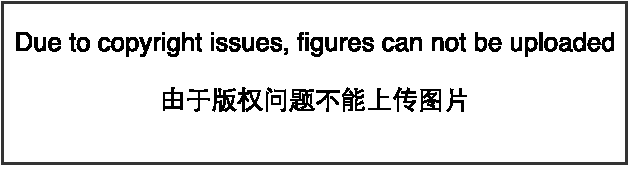
\includegraphics{figure.pdf}}
\else
\centerline{\includegraphics{Chapter5/figures/underfit_just_right_overfit_color}}
\fi
\caption{TODO}
\label{fig:chap5_underfit_just_right_overfit}
\end{figure}

% -- 109 --

目前为止,我们只探讨了可以通过改变输入\gls{feature}的数目,同时加入这些\gls{feature}对应的参数,去改变模型的容量。
事实上有很多方法改变模型的容量。
容量不仅取决于模型的选择。
模型规定了当调整参数降低训练对象时,学习算法可以从哪些函数族中选择函数。
这被称为模型的\firstgls{representational_capacity}。
在很多情况下,从这些函数中挑选出最优函数是非常困难的优化问题。
实际中,学习算法不会真的找到最优函数,而仅是找到一个可以降低训练误差很多的函数。
这些额外的限制因素,比如优化算法的不完美,意味着学习算法的\firstgls{effective_capacity}可能小于模型族的\gls{representational_capacity}。

% -- 110 --

关于提高\gls{ML}模型泛化的现代思想可以追溯到早在托勒密时期的哲学家的思想。
许多早期的学者引用的简约原则,现在被广泛称为\firstgls{OR}(c. 1287-1387)。
该原则指出,同样能够解释已知观测现象的假设中,我们应该挑选“最简单”的那一个。
这个想法是在20世纪,由统计学习理论创始人提出来并精确化的\citep{Vapnik71,Vapnik82,Blumer-et-al-1989,Vapnik95}。

统计学习理论提供了量化模型容量的不同方法。
在这些中,最有名的是\firstall{VC}。
\gls{VC}衡量二元分类器的容量。
\gls{VC}定义为该分类器能够分类的训练\gls{example:chap5}的最多数目。
假设存在$m$个不同$\Vx$点的训练集,分类器可以任意地标记该$m$个不同的$\Vx$点,\gls{VC}被定义为$m$的最大可能值。

量化模型的容量使得统计学习理论可以进行量化预测。
统计学习理论中最重要的结论阐述了训练误差和泛化误差之间差异的上界随着模型容量增长而增长,但随着训练\gls{example:chap5}增多而下降\citep{Vapnik71,Vapnik82,Blumer-et-al-1989,Vapnik95}。
这些边界为\gls{ML}算法可以有效解决问题提供了理论验证,但是它们很少应用于实际中的\gls{DL}算法。
一部分原因是边界太松,另一部分原因是很难确定\gls{DL}算法的容量。
确定\gls{DL}模型容量的问题特别困难是由于有效容量受限于优化算法的能力。
我们只有很少的理论分析\gls{DL}中出现的一般非凸优化问题。

我们必须记住虽然更简单的函数更可能泛化(训练误差和测试误差的差距小),但我们仍然需要选择一个充分复杂的假设以达到低的\gls{training_error}。
通常,当模型容量上升(假设误差衡量有最小值)时,训练误差会下降,直到其渐近最小可能误差。
通常,\gls{generalization_error}是一个关于模型容量U形曲线函数。
如图\ref{fig:chap5_generalization_vs_capacity}所示。

\begin{figure}[!htb]
\ifOpenSource
\centerline{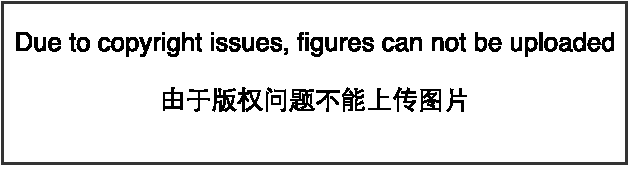
\includegraphics{figure.pdf}}
\else
\centerline{\includegraphics{Chapter5/figures/generalization_vs_capacity_color}}
\fi
\caption{TODO}
\label{fig:chap5_generalization_vs_capacity}
\end{figure}

% -- 111 --

考虑任意高容量的极端情况,我们介绍\firstgls{nonparametric}\emph{模型}的概念。
至此,我们只探讨过参数模型,例如\gls{linear_regression}。
参数模型学习到的函数在观测新数据前,参数是有限且固定的向量。
非参数模型没有这些限制。

有时,非参数模型仅是一些不能实际实现的理论抽象(比如搜索所有可能概率分布的算法)。
然而,我们也可以设计一些实用的非参模型,使它们的复杂度和训练集大小有关。
这种算法的一个示例是\firstgls{nearest_neighbor_regression}。
不像\gls{linear_regression}有固定长度的向量作为权重,\gls{nearest_neighbor_regression}模型简单地存储了训练集中的$\MX$和$\Vy$。
当需要为测试点$\Vx$分类时,模型会查询训练集中离该点最近的点,并返回相关的回归\gls{target}。
换言之,$\hat{y}=y_i$其中$i=\argmin\norm{\MX_{i,:}-\Vx}_2^2$。
该算法也可以扩展成$L^2$范数以外的距离度量,例如学习距离度量\citep{RoweisNCA2005}。
如果该算法通过平均$\MX_{i,:}$中所有最近的向量对应的$y_i$来打破平局,那么该算法会在任意回归\gls{dataset}上达到最小可能的训练误差(如果存在两个相同的输入对应不同的输出,那么训练误差可能会大于零)。

最后,我们也可以将参数学习算法嵌入另一个依所需增加参数数目的算法来创建非参数学习算法。
例如,我们可以想象外层循环调整多项式的次数,内存循环通过\gls{linear_regression}学习模型。

% -- 112 --

理想模型假设我们能够预先知道生成数据的真实概率分布。
尽管这样的模型仍然会在很多问题上发生一些错误,因为分布中仍然会有一些噪音。
在\gls{supervised_learning}中,从$\Vx$到$y$的映射可能内在是随机的,或者$y$可能是包括$\Vx$在内还有其他变量的确定性函数。
假设预先知道,从真实分布$p(\Vx,y)$预测而出现的误差被称为\firstgls{bayes_error}。

\gls{training_error}和\gls{generalization_error}会随训练集的大小发生变化。
泛化误差的期望不会随着训练\gls{example:chap5}数目的增加而增加。
对于非参数模型而言,更多的数据会得到更好的泛化能力,直到达到最佳可能的泛化误差。
任何模型容量小于最优容量的固定参数模型会渐近到大于\gls{bayes_error}的误差值。
如图\ref{fig:chap5_training_size_grows}所示。
值得注意的是,具有最优容量的模型仍然有可能在\gls{training_error}和\gls{generalization_error}之间存在很大的差距。
在这种情况下,我们可以通过收集更多的训练\gls{example:chap5}来缩小差距。

\begin{figure}[!htb]
\ifOpenSource
\centerline{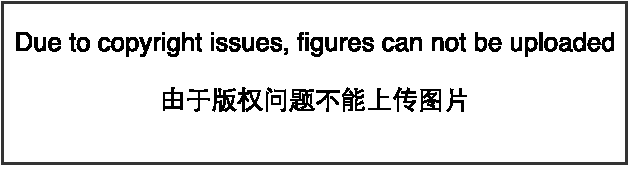
\includegraphics{figure.pdf}}
\else
\centerline{\includegraphics{Chapter5/figures/training_size_grows}}
\fi
\caption{TODO}
\label{fig:chap5_training_size_grows}
\end{figure}

\subsection{\glsentrytext{no_free_lunch_theorem}}
\label{sec:the_no_free_lunch_theorem}
学习理论表明\gls{ML}算法能够从有限个训练集\gls{example:chap5}中很好地泛化。
这似乎违背一些基本的逻辑原则。
归纳推理,或是从一组有限的\gls{example:chap5}中推断一般的规则,在逻辑上不是很有效。
逻辑地推断一个规则去描述集合中的元素,我们必须对集合中的每个元素都有信息。

在一定程度上,\gls{ML}只是通过概率法则就可以避免这个问题,而不是使用纯逻辑推理的整个确定性法则。
\gls{ML}保证找到一个所关心的 \emph{大多数}\gls{example:chap5}\emph{可能}正确的规则。

不幸的是,即使这样也不能解决整个问题。
\gls{ML}的\firstgls{no_free_lunch_theorem}表明,在所有可能的数据生成分布上平均,每一个分类算法在未事先观测的点上都有相同的错误率。
换言之,某种意义上,没有一个\gls{ML}算法总是比其他的要好。
我们能够设想的最先进的算法和仅仅将每一个点归为同一类的简单算法有着相同的平均性能(在所有可能的任务上)。

% -- 113 --

幸运的是,这些结论仅在我们考虑所有可能的数据生成分布时才成立。
在现实世界的应用中,如果我们对遇到的概率分布的种类进行假设的话,那么我们可以设计在这些分布上效果良好的学习算法。

这意味着\gls{ML}研究的\gls{target}不是找一个通用学习算法或是绝对最好的学习算法。
反之,我们的\gls{target}是理解什么样的分布和人工智能体验的“真实世界”相关,什么样的学习算法在我们关心的数据生成分布上效果最好。

\subsection{\glsentrytext{regularization}}
\label{sec:regularization}
没有免费午餐定理暗示我们必须设计在特定任务上效果良好的\gls{ML}算法。
我们建立一组学习算法的偏好来达到这个要求。
当这些偏好和我们希望算法解决的学习问题相吻合时,性能会更好。

至此,我们讨论修改学习算法的唯一方法是通过增加或减少学习算法可选假设空间的函数来增加或减少模型的容量。
我们列举的一个具体例子是\gls{linear_regression}中增加或减少多项式的次数。
我们目前为止讨论的观点都是过度简化的。

我们算法的效果不仅受影响于假设空间的函数数量,也取决于这些函数的具体形式。
我们已经讨论的学习算法,\gls{linear_regression},的假设空间包含关于输入的线性函数集。
这些线性函数对于输入和输出确实接近线性相关的问题是很有用的。
对于完全非线性的问题他们没有什么效果。
例如,如果我们尝试用\gls{linear_regression}从$x$去预测$\sin(x)$,效果不会好。
我们控制算法的性能,可以通过控制允许采样的函数种类,也可以通过控制这些函数的数量。

在假设空间中,我们可以偏好一个学习算法,相比于另一个算法。
这意味着两个函数都是符合条件的,但是我们更偏好其中一个。
只有在不被偏好的函数比偏好的在训练\gls{dataset}上效果好得非常明显的时候,我们才会考虑不被偏好的。

% -- 115 --

例如,我们可以加入\firstgls{weight_decay}来修改\gls{linear_regression}的训练标准。
带权重衰减的\gls{linear_regression}最小化包含训练集上的最小均方差和规则项的和$J(\Vw)$,偏好于平方$L^2$范数较小的权重。
具体如下:
\begin{equation}
    J(\Vw) = \text{MSE}_{\text{train}} + \lambda \Vw^\Tsp \Vw,
\end{equation}
其中$\lambda$是提前挑选的值,控制我们偏好小范数权重的程度。
当$\lambda =0$,我们没有任何偏好。
越大的$\lambda$偏好范数越小的权重。
最小化$J(\Vw)$可以看作是在拟合训练数据和使权重范数小之间的权衡。
这会使得解决方案的斜率较小,或是将权重放在较少的\gls{feature}上。
我们可以训练带不同$\lambda$之的高次多项式来举例说明如何通过权重衰减来控制模型欠拟合或过拟合的趋势。
如图\ref{fig:chap5_underfit_just_right_overfit_wd_color}所示。

\begin{figure}[!htb]
\ifOpenSource
\centerline{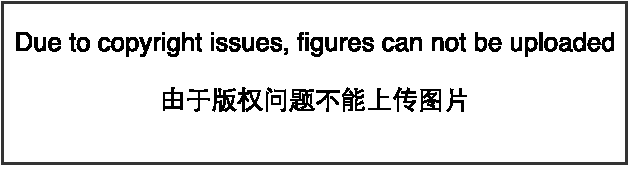
\includegraphics{figure.pdf}}
\else
\centerline{\includegraphics{Chapter5/figures/underfit_just_right_overfit_wd_color}}
\fi
\caption{TODO}
\label{fig:chap5_underfit_just_right_overfit_wd_color}
\end{figure}

更一般地,\gls{regularization}一个学习函数$f(\Vx;\Vtheta)$的模型,我们可以给损失函数添加称为\firstgls{regularizer}的惩罚。
在权重衰减的例子中,\gls{regularizer}是$\Omega(\Vw) = \Vw^\Tsp \Vw$。在第\ref{chap:regularization_for_deep_learning}章,我们将看到很多其他可能的\gls{regularizer}。

% -- 116 --

表示对函数的偏好是比增减假设空间的成员函数更一般的去控制模型\gls{capacity}的方法。
我们可以将从假设空间中去掉某个函数看作是对这个函数的无限偏好。

在我们权重衰减的示例中,通过在最小化的\gls{target}中额外增加一项,我们明确地表示了偏好权重较小的线性函数。
有很多其他方法去隐式地或显式地表示对不同解决方法的偏好。
总的来说,这些不同的方法都被称为\firstgls{regularization}。
\emph{\gls{regularization}是指我们对学习算法所做的趋向于降低泛化误差而非训练误差的修改}。
\gls{regularization}是\gls{ML}领域的中心问题之一,能够和其重要性媲美的只有优化。

\gls{no_free_lunch_theorem}已经清楚阐述了没有最优的学习算法,特别地,没有最优的\gls{regularization}形式。
反之,我们必须挑选一个非常适合于我们要解决任务的正则形式。
\gls{DL}中普遍的,特别是本书的,理念是大量任务(例如所有人类能做的智能任务)也许都可以使用非常通用的\gls{regularizer}来有效解决。

\section{超参数和验证集}
\label{sec:hyperparameters_and_validation_sets}
大多数\gls{ML}算法具有超参数,我们可以用来控制算法行为的设置。
超参数的值不是通过学习算法本身拟合出来的(尽管我们可以设计一个嵌套的学习过程,一个学习算法为另一个学习算法学出最优超参数)。

在图5.2所示的多项式回归实例中,有一个超参数:多项式的次数,作为\textbf{\gls{capacity}}超参数。
控制\gls{weight_decay}程度的$\lambda$是另一个超参数。

有时一个\gls{setting}被设为学习算法不用学习的超参数,是因为它太难优化了。
更经常地,如果某个\gls{setting}不适合在训练集上学习,那么它必须被设为超参数。
这适用于控制模型\gls{capacity}的所有超参数。
如果在训练集上学习超参数,这些超参数总是趋向于最大可能的模型容量,导致过拟合(参考图5.3)。
例如,相较低次多项式和正的权重衰减设定,更高次的多项式和权重衰减参数设定为$\lambda=0$总能在训练集上更好地拟合。

% -- 117 --

为了解决这个问题,我们需要训练算法观测不到的\firstgls{validation_set}\gls{example:chap5}。

早先我们讨论过和训练数据相同分布的\gls{example:chap5}组成的\gls{test_set}可以用来估计学习过程完成之后的学习器的泛化误差。
其重点在于测试\gls{example:chap5}不能以任何形式参与到模型的选择,包括设定超参数。
基于这个原因,\gls{test_set}中的\gls{example:chap5}不能用于验证集。
因此,我们总是从\emph{训练}数据中构建验证集。
特别地,我们将训练数据分成两个不相交的子集。
其中一个用于学习参数。
另外一个便是我们的验证集,用于估计训练中或训练后的泛化误差,使超参数相应地更新。
用于学习参数的数据子集通常仍被称为训练集,尽管这会和整个训练过程用到的更大的\gls{dataset}相混。
用于挑选超参数的数据子集被称为\gls{validation_set}。
通常,$80\%$的训练数据用于训练,$20\%$用于验证。
由于验证集是用来“训练”超参数的,尽管验证集的误差通常会比训练集误差小,验证集会低估泛化误差。
所有超参数优化完成之后,泛化误差可能通过\gls{test_set}来估计。

在实际中,当相同的\gls{test_set}已经重复地用于评估不同算法的性能很多年,特别是如果我们考虑来自学术界的各种尝试去挑战该\gls{test_set}上报道出来的最佳性能,我们最后也会对\gls{test_set}有着乐观的估计。
\gls{benchmarks}会因之变得陈旧,而后不能反映训练系统的真实性能。
值得庆幸的是,学术界往往会移到新的(通常会更具大更具挑战性的)基准\gls{dataset}上。

\subsection{交叉验证}
\label{sec:cross_validation}
将\gls{dataset}分成固定的训练集和固定的\gls{test_set}后,若\gls{test_set}的误差很小,这将是有问题的。
一个小规模的\gls{test_set}意味着平均测试误差估计的统计不确定性,使得很难判断算法$A$是否比算法$B$在给定的任务上做得更好。

% -- 118 --

当\gls{dataset}有十万计或者更多的\gls{example:chap5}时,这不会是一个严重的问题。
当\gls{dataset}太小时,也有替代方法允许我们使用所有的\gls{example:chap5}估计平均测试误差,代价是增加了计算量。
这些过程是基于在原始数据随机采样或分离出的不同\gls{dataset}上重复训练和测试计算的想法。
最常见的是$k$折交叉验证过程,如算法5.1所示,将\gls{dataset}分成$k$个不重合的子集。
测试误差可以估计为$k$次计算后的平均测试误差。
在第$i$次测试时,数据的第$i$个子集用于\gls{test_set},其他的数据用于训练集。
一个问题是不存在平均误差方差的无偏估计\citep{Bengio-Grandvalet-JMLR-04},但是我们通常会使用近似。

\section{估计,偏差和方差}
\label{sec:estimators_bias_and_variance}
统计领域为我们提供了很多工具用于实现\gls{ML}目标,不仅可以解决训练集上的任务,还可以泛化。
基本的概念,例如参数估计,偏差和方差对于形式化刻画泛化,欠拟合和过拟合都非常有帮助。

\subsection{点估计}
\label{sec:point_estimation}
点估计试图为一些感兴趣的量提供单个“最优”预测。
一般地,感兴趣的量可以是单个参数,或是某些参数模型中一个向量参数,例如第5.1.4节\gls{linear_regression}中的权重,但是也有可能是整个函数。

为了区分参数估计和真实值,我们习惯表示参数$\Vtheta$的点估计为$\hat{\Vtheta}$。

让$\{\Vx^{(1)},\dots,\Vx^{(m)}\}$是$m$个独立同分布(i.i.d.)的数据点。
\firstgls{point_estimator}或\firstgls{statistics}是这些数据的任意函数:
\begin{equation}
    \hat{\Vtheta}_m = g(\Vx^{(1)}, \dots, \Vx^{(m)}) .
\end{equation}
这个定义不要求$g$返回一个接近真实植$\Vtheta$的值,或是$g$的值域为$\Vtheta$的允许取值。
点估计的定义非常宽泛,给了\gls{estimator:chap5}的设计者极大的灵活性。
虽然几乎所有函数都可以称为\gls{estimator:chap5},但是一个好的\gls{estimator:chap5}的输出会接近生成训练数据的真实参数$\Vtheta$。

% -- 119 --

现在,我们采取频率派在统计上的观点。
换言之,我们假设真实参数$\Vtheta$是固定但未知的,而点估计$\hat{\Vtheta}$是数据的函数。
由于数据是随机过程采样出来的,数据的任何函数都是随机的。
因此$\hat{\Vtheta}$是一个随机变量。

% -- 120 --

点估计也可以指输入和\gls{target}变量之间关系的估计。
我们将这类点估计称为函数估计。

\textbf{函数估计}\quad 有时我们会关注函数估计(或函数近似)。
这时我们试图从输入向量$\Vx$预测变量$\Vy$。
我们假设有一个函数$f(\Vx)$表示$\Vy$和$\Vx$之间的近似关系。
例如,我们可能假设$\Vy = f(\Vx) + \Vepsilon$,其中$\Vepsilon$是$\Vy$中未能从$\Vx$预测的一部分。
在函数估计中,我们感兴趣的是用模型估计去近似$f$,或者估计$\hat{f}$。
函数估计和估计参数$\Vtheta$是一样的;函数估计$\hat{f}$是函数空间中的一个点估计。
\gls{linear_regression}实例(第5.1.4节中讨论的)和多项式回归实例(第5.2节中讨论的)都既可以被解释为估计参数$\Vw$,又可以解释为估计从$\Vx$到$y$的函数映射$\hat{f}$。

现在我们回顾点估计最常研究的性质,并探讨这些性质说明了估计的什么。

\subsection{偏差}
\label{sec:bias}
估计的偏差被定义为:
\begin{equation}
\label{eq:5.20}
    \text{bias}(\hat{\Vtheta}_m) = \SetE(\hat{\Vtheta}_m) - \Vtheta,
\end{equation}
其中期望作用在所有数据(看作是从随机变量采样得到的)上,$\Vtheta$是定义数据生成分布$\Vtheta$的真实值。
如果$\text{bias}(\hat{\Vtheta}_m)=0$,那么\gls{estimator:chap5}$\hat{\Vtheta}_m$被称为是\firstgls{unbiased},这意味着$\SetE(\hat{\Vtheta}_m) = \Vtheta$。
如果$\lim_{m\to\infty} \text{bias}(\hat{\Vtheta}_m)=0$,那么\gls{estimator:chap5}$\hat{\Vtheta}_m$称为是\firstgls{asymptotically_unbiased},这意味着$\lim_{m\to\infty} \SetE(\hat{\Vtheta}_m) = \Vtheta$。

% -- 121 --

\textbf{实例:伯努利分布}\quad 
考虑一组服从均值为$\theta$的伯努利分布的独立同分布采样$\{x^{(1)}, \dots , x^{(m)}\}$:
\begin{equation}
    P(x^{(i)}; \theta) = \theta^{x^{(i)}} (1-\theta)^{(1 - x^{(i)})}.
\end{equation}
这个分布中参数$\theta$的常用估计是训练\gls{example:chap5}的均值:
\begin{equation}
\label{eq:5.22}
    \hat{\theta}_m = \frac{1}{m} \sum_{i=1}^m x^{(i)}.
\end{equation}
判断这个\gls{estimator:chap5} 是否有偏,我们将式\ref{eq:5.22}代入式\ref{eq:5.20}:
\begin{align}
    \text{bias}(\hat{\theta}_m)     &= \SetE[\hat{\theta}_m] - \theta  \\
            &= \SetE \left[ \frac{1}{m} \sum_{i=1}^m x^{(i)} \right] - \theta \\
            &= \frac{1}{m} \sum_{i=1}^m \SetE \left[x^{(i)} \right] - \theta \\
            &= \frac{1}{m} \sum_{i=1}^m \sum_{x^{(i)} = 0}^1 \left( x^{(i)} \theta^{x^{(i)}} (1-\theta)^{(1-x^{(i)})} \right) - \theta \\
            &= \frac{1}{m} \sum_{i=1}^m (\theta) - \theta \\
            &= \theta - \theta = 0
\end{align}

因为$\text{bias}(\hat{\theta})=0$,我们称估计$\hat{\theta}$是无偏的。

\textbf{实例:均值的高斯分布估计}\quad 
现在,考虑一组独立同分布的\gls{example:chap5}$\{x^{(1)}, \dots , x^{(m)}\}$服从高斯分布$p(x^{(i)}) = \mathcal{N}(x^{(i)}; \mu, \sigma^2)$,其中$i\in\{1, \dots, m\}$。
回顾高斯概率密度函数如下:
\begin{equation}
    p(x^{(i)}; \mu, \sigma^2) = \frac{1}{\sqrt{2\pi\sigma^2}} \exp\left( -\frac{1}{2} \frac{(x^{(i)} - \mu)^2}{\sigma^2}  \right).
\end{equation}

高斯均值参数的常用\gls{estimator:chap5}被称\firstgls{sample_mean}:
\begin{equation}
    \hat{\mu}_m = \frac{1}{m} \sum_{i=1}^m x^{(i)}
\end{equation}
判断\gls{sample_mean}是否有偏,我们再次计算它的期望:
\begin{align}
\text{bias} (\hat{\mu}_m) &= \SetE[ \hat{\mu}_m ]  - \mu \\
    &= \SetE \left[ \frac{1}{m} \sum_{i=1}^m x^{(i)}  \right] - \mu \\
    &= \left( \frac{1}{m}\sum_{i=1}^m \SetE \left[ x^{(i)} \right] \right) - \mu \\
    &= \left( \frac{1}{m}\sum_{i=1}^m \mu \right) - \mu \\
    &= \mu - \mu = 0
\end{align}
因此我们发现\gls{sample_mean}是高斯均值参数的无偏\gls{estimator:chap5}。

% -- 122 --

\textbf{实例:高斯分布方差估计}\quad 
本例中,我们比较高斯分布方差参数$\sigma^2$的两个不同估计。
我们探讨是否有一个是有偏的。

我们考虑的第一个方差估计称为\firstgls{sample_variance}:
\begin{equation}
    \hat{\sigma}_m^2 = \frac{1}{m} \sum_{i=1}^m \left( x^{(i)} - \hat{\mu}_m \right)^2,
\end{equation}
其中$\hat{\mu}_m$是\gls{sample_variance}。
更形式地,我们感兴趣计算
\begin{equation}
\label{eq:5.37}
    \text{bias} (\hat{\sigma}_m^2) = \SetE [ \hat{\sigma}_m^2 ]  - \sigma^2.
\end{equation}
我们首先估计项$\SetE [ \hat{\sigma}_m^2 ]$:
\begin{align}
    \SetE [ \hat{\sigma}_m^2 ]  &= \SetE \left[ \frac{1}{m} \sum_{i=1}^m \left( x^{(i)} - \hat{\mu}_m \right)^2  \right] \\
    &= \frac{m-1}{m} \sigma^2
\end{align}
回到式\ref{eq:5.37},我们得到结论$\hat{\sigma}^2_m$的偏差是$-\frac{\sigma^2}{m}$。
因此\gls{sample_variance}是有偏估计。

\firstgls{unbiased_sample_variance}估计
\begin{equation}
    \tilde{\sigma}_m^2 = \frac{1}{m-1} \sum_{i=1}^m \left( x^{(i)} - \hat{\mu}_m \right)^2
\end{equation}
提供了另一种可选方法。
正如名字所说,这个估计是无偏的。
换言之,我们会发现$\SetE[\tilde{\sigma}_m^2] = \sigma^2$:
\begin{align}
    \SetE[\tilde{\sigma}_m^2] &= \SetE \left[ \frac{1}{m-1} \sum_{i=1}^m \left( x^{(i)} - \hat{\mu}_m \right)^2 \right] \\
        &= \frac{m}{m-1} \SetE[ \hat{\sigma}_m^2 ]  \\
        &= \frac{m}{m-1} \left( \frac{m-1}{m} \sigma^2 \right) \\
        &= \sigma^2.
\end{align}

% -- 123 --

我们有两个\gls{estimator:chap5}:一个是有偏的,另一个是无偏的。
尽管无偏估计显然是可取的,但它并不总是“最好”的估计。
我们将会看到经常会使用具有其他重要性质的有偏估计。

\subsection{方差和\glsentrytext{standard_error}}
\label{sec:variance_and_standard_error}
我们可能要考虑的\gls{estimator:chap5}另一个性质是数据样本函数的变化程度。
正如我们可以计算\gls{estimator:chap5}的期望去决定它的偏差,我们也可以计算它的方差。
\gls{estimator:chap5}的\firstgls{variance}就是一个\gls{variance}
\begin{equation}
    \text{Var}(\hat{\theta})
\end{equation}
其中随机变量是训练集。
另外,方差的平方根被称为\firstgls{standard_error},记作$\text{SE}(\hat{\theta})$。

\gls{standard_error}的方差或\gls{standard_error}提供给我们,当\gls{dataset}独立地从潜在的数据生成过程中重采样数据集时,如何期望估计的变化。
正如我们希望估计的偏差比较小,我们也希望其方差较小。

当我们使用有限的样本计算任何统计量时,真实参数的估计都是不确定的,在这个意义下,从相同的分布得到其他样本时,它们的统计量会不一样。
任何估计方差的期望程度是我们想量化的误差的来源。

均值的\gls{standard_error}被记作
\begin{equation}
\label{eq:5.46}
    \text{SE}(\hat{\mu}_m) = \sqrt{ \text{Var} \left[ \frac{1}{m} \sum_{i=1}^m x^{(i)} \right] } = \frac{\sigma}{\sqrt{m}},
\end{equation}
其中$\sigma^2$是\gls{example:chap5}$x^i$的真实方差。
\gls{standard_error}通常被记作$\sigma$。
不幸的是,样本方差的平方根和方差无偏估计的平方根都不是\gls{standard_deviation}的无偏估计。
这两种计算方法都倾向于低估真实的\gls{standard_deviation},但仍用于实际中。
方差无偏估计的平方根是不太低估的。
对于较大的$m$,这种近似非常合理。

% -- 124 --

均值的\gls{standard_error}在\gls{ML}实验中非常有用。
我们通常计算\gls{test_set}误差的样本均值来估计泛化误差。
\gls{test_set}中\gls{example:chap5}的数量决定了这个估计的精确度。
中心极限定理告诉我们均值会接近一个高斯分布,我们可以用\gls{standard_error}计算出真实期望落在选定区间的概率。
例如,以均值$\hat{\mu}_m$为中心的$95\%$置信区间是
\begin{equation}
    ( \hat{\mu}_m - 1.96\text{SE}(\hat{\mu}_m), \hat{\mu}_m + 1.96 \text{SE}(\hat{\mu}_m) ),
\end{equation}
以上区间基于均值是$\hat{\mu}_m$和方差$\text{SE}(\hat{\mu}_m)^2$的高斯分布。
在\gls{ML}实验中,我们通常说算法$A$比算法$B$好,是指算法$A$的误差的$95\%$置信区间的上界小于算法算法$B$的误差的$95\%$置信区间的下界。

\textbf{实例:伯努利分布} \quad 我们再次考虑从伯努利分布(回顾$P(x^{(i)}; \theta) = \theta^{x^{(i)}} (1-\theta)^{1 - x^{(i)}}$)中独立同分布采样出来的一组\gls{example:chap5}$\{ x^{(1)}, \dots, x^{(m)} \}$。
这次我们关注估计$\hat{\theta}_m = \frac{1}{m} \sum_{i=1}^m x^{(i)}$的方差:
\begin{align}
    \text{Var}\left( \hat{\theta}_m \right) &= \text{Var}\left( \frac{1}{m} \sum_{i=1}^m x^{(i)} \right) \\
    &= \frac{1}{m^2} \sum_{i=1}^m \text{Var} \left( x^{(i)} \right) \\
    &= \frac{1}{m^2} \sum_{i=1}^m \theta (1 - \theta) \\
    &= \frac{1}{m^2} m\theta(1-\theta) \\
    &= \frac{1}{m} \theta(1-\theta)
\end{align} 
估计方差以\gls{dataset}\gls{example:chap5}数目$m$的函数方式下降。
这是估计普遍的共同性质,在探讨一致性(参考第5.4.5节)时,我们会继续讨论。

% -- 125 --

\subsection{权衡偏值和方差以最小化均方误差}
\label{sec:trading_off_bias_and_variance_to_minimize_mean_squared_error}
偏差和方差衡量估计的两个不同误差来源。
偏差衡量离真实函数或参数的误差期望。
另一方面,方差衡量由任意特定的数据采样可能导致的估计期望的偏差。

当可以选择一个偏差更大的估计和一个方差更大的估计时,会发生什么呢?我们如何选择?
例如,想象我们希望近似图5.2中的函数,我们只可以选择一个偏差较大的估计或一个方差较大的估计,我们该如何选择呢?

判断这种权衡最常用的方法是交叉验证。
经验上,交叉验证在许多真实世界的任务中都非常成功。
另外,我们也可以比较这些估计的\firstall{mean_squared_error}:
\begin{align}
    \text{MSE} &= \SetE[ ( \hat{\theta}_m - \theta  )^2 ] \\
        &= \text{Bias}( \hat{\theta}_m )^2 + \text{Var}( \hat{\theta}_m ) \label{eq:5.54}
\end{align}
MSE衡量估计和真实参数$\theta$之间使用平方误差的总体期望偏离。
如式\ref{eq:5.54}所示,MSE估计包含了偏差和方差。
理想的估计具有较小的MSE或是在检查中会稍微约束它们的偏差和方差。

偏差和方差的关系和\gls{ML}容量,欠拟合和过拟合的概念紧密相连。
用MSE衡量泛化误差(偏差和方差对于泛化误差都是有意义的)时,增加容量会增加方差,降低偏差。
如图\ref{fig:chap5_bias_variance_tradeoff}所示,我们会再次看到容量函数泛化误差的U形曲线。

\begin{figure}[!htb]
\ifOpenSource
\centerline{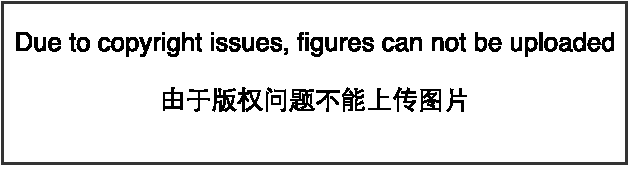
\includegraphics{figure.pdf}}
\else
\centerline{\includegraphics{Chapter5/figures/bias_variance_tradeoff}}
\fi
\caption{TODO}
\label{fig:chap5_bias_variance_tradeoff}
\end{figure}

% -- 126 --

\subsection{一致性}
\label{sec:consistency}
目前我们已经探讨了固定大小训练集下不同估计的性质。
通常,我们也会关注训练数据增多后估计的性能。
特别地,我们希望当\gls{dataset}中数据点的数量$m$增加时,点估计会收敛到对应参数的真实值。
更形式地,我们想要
\begin{equation}
\label{eq:5.55}
    \plim_{m\to\infty} \hat{\theta}_m = \theta.
\end{equation}
符号$\plim$表示依概率收敛,即对于任意的$\epsilon > 0$,当$m\to\infty$时,有$P(|\hat{\theta}_m - \theta| > \epsilon) \to 0$。
式\ref{eq:5.55}表示的条件被称为\firstgls{consistency}。
它有时候是指弱一致性,强一致性是指\firstgls{almost_sure}从$\hat{\theta}$收敛到$\theta$。
\firstgls{almost_sure_convergence}是指当$p(\lim_{m\to\infty} \RVx^{(m)} = \Vx) = 1 $时,随机变量序列$\RVx^{(1)}$,$\RVx^{(2)}$,$\dots$收敛到$\Vx$。

一致性保证了估计偏差会随数据\gls{example:chap5}数目的增多而减少。
然而,反过来不是正确的----渐近无偏并不意味着一致性。
例如,考虑用包含$m$个样本的\gls{dataset}$\{x^{(1)},\dots,x^{(m)}\}$估计正态分布$\mathcal{N}(x;\mu,\sigma^2)$的均值参数$\mu$。
我们可以使用\gls{dataset}的第一个\gls{example:chap5}$x^{(1)}$作为无偏(unbiased)估计:$\hat{\theta} = x^{(1)}$。
在该情况下,$\SetE(\hat{\theta}_m) = \theta$,所以不管观测到多少数据点,该估计都是无偏的。
然而,这不是一个一致性估计,因为它\emph{不}满足当$m\to\infty$时,$\hat{\theta}_m \to \theta$。

% -- 127 --

\section{\glsentrytext{maximum_likelihood_estimation}}
\label{sec:maximum_likelihood_estimation}
之前,我们已经看过常用估计的定义,并分析了它们的性质。
但是这些估计是从哪里来的呢?
并非猜测某些函数可能是好的估计,然后分析其偏差和方差,我们希望有些准则可以让我们从不同模型中得到特定函数作为好的估计。

最常用的准则是\gls{maximum_likelihood_estimation}。

考虑一组含有$m$个\gls{example:chap5}的\gls{dataset}$\SetX=\{ \Vx^{(1)},\dots, \Vx^{(m)} \}$,独立地由真正但未知的数据生成分布$p_{\text{data}}(\RVx)$生成。

让$p_{\text{model}}( \RVx; \Vtheta )$是一族由$\Vtheta$确定在相同空间上的概率分布。
换言之,$p_{\text{model}}(\Vx;\Vtheta)$将任意输入$\Vx$映射到实数去估计真实概率$p_{\text{data}}(\Vx)$

 $\Vtheta$的最大后验估计被定义为:
\begin{align}
    \Vtheta_{\text{ML}} &= \underset{\Vtheta}{\argmax} p_{\text{model}} (\SetX; \Vtheta), \\
        &= \underset{\Vtheta}{\argmax} \prod_{i=1}^m p_{\text{model}} (\Vx^{(i)}; \Vtheta).
\end{align}

很多概率的乘积会因很多原因不方便。
例如,很容易出现数值下溢。
为了得到一个更方便但是等价的优化问题,我们观察到似然对数不会改变其$\argmax$但是便利地将乘积转化成了和:
\begin{equation}
    \Vtheta_{\text{ML}} = \underset{\Vtheta}{\argmax} \sum_{i=1}^m \log p_{\text{model}} (\Vx^{(i)}; \Vtheta) .
\end{equation}
因为当我们重新缩放损失函数时$\argmax$不会改变,我们可以除以$m$得到和训练数据经验分布$\hat{p}_{\text{data}}$相关的期望作为准则:
\begin{equation}
\label{eq:5.59}
    \Vtheta_{\text{ML}} = \underset{\Vtheta}{\argmax} \SetE_{\RVx \sim \hat{p}_{\text{data}}} \log p_{\text{model}} (\Vx; \Vtheta) .
\end{equation}

解释\gls{maximum_likelihood_estimation}的一种观点是将它看作最小化训练集上的经验分布$\hat{p}_{\text{data}}$和模型分布之的间差异,两者之间的差异程度可以通过KL散度衡量。
KL散度定义为
\begin{equation}
    D_{\text{KL}}(\hat{p}_{\text{data}} || p_{\text{model}}) = \SetE_{\RVx \sim \hat{p}_{\text{data}}} [ \log \hat{p}_{\text{data}}(\Vx) - \log p_{\text{model}}(\Vx) ] .
\end{equation}
左边一项仅涉及到数据生成过程,和模型无关。
这意味着当我们训练模型最小化KL散度时,我们只需要最小化
\begin{equation}
    -\SetE_{\RVx \sim \hat{p}_{\text{data}}} [ \log p_{\text{model}}(\Vx)  ] ,
\end{equation}
当然,这和式\ref{eq:5.59}中最大化是相同的。

% -- 128 --

最小化KL散度其实就是在最小化分布之间的交叉熵。
许多作者使用术语“交叉熵”特定表示伯努利或softmax分布的负对数似然,但那是用词不当的。
任何一个由负对数似然组成的损失都是定义在训练集上的经验分布和定义在模型上的概率分布之间的交叉熵。
例如,\gls{mean_squared_error}是经验分布和高斯模型之间的交叉熵。

我们可以将最大似然看作是使模型分布尽可能和经验分布$\hat{p}_{\text{data}}$相匹配的尝试。
理想情况下,我们希望匹配真实的数据生成分布$p_{\text{data}}$,但我们没法直接知道这个分布。

虽然最优$\Vtheta$在最大化似然或是最小化KL散度时是相同的,但是目标函数值是不一样的。
在软件中,我们通常将两者都称为最小化损失函数。
因此最大化似然变成了最小化负对数似然(NLL),或者等价的是最小化交叉熵。
将最大化似然看作最小化KL散度的视角在这个情况下是有帮助的,因为已知KL散度最小值是零。
当$\Vx$取实数时,负对数似然是负值。

\subsection{条件对数似然和\glsentrytext{mean_squared_error}}
\label{sec:conditional_log_likelihood_and_mean_squared_error}
\gls{maximum_likelihood_estimation}很容易扩展到估计条件概率$P(\Vy|\Vx;\Vtheta)$,给定$\Vx$预测$\Vy$。
实际上这是最常见的情况,因为这构成了大多数\gls{supervised_learning}的基础。
如果$\MX$表示所有的输入,$\MY$表示我们观测到的\gls{target},那么条件\gls{maximum_likelihood_estimation}是
\begin{equation}
    \Vtheta_{\text{ML}} = \underset{\Vtheta}{\argmax} P(\MY | \MX; \Vtheta).
\end{equation}
如果假设\gls{example:chap5}是独立同分布的,那么这可以分解成
\begin{equation}
\label{eq:5.63}
    \Vtheta_{\text{ML}} = \underset{\Vtheta}{\argmax} \sum_{i=1}^m \log P(\Vy^{(i)} | \Vx^{(i)}; \Vtheta).
\end{equation}

% -- 129 --

\textbf{实例:\gls{linear_regression}作为最大似然}\quad 第5.1.4节介绍的\gls{linear_regression},可以被看作是最大似然过程。
之前,我们将\gls{linear_regression}作为学习从输入$\Vx$映射到输出$\hat{y}$的算法。
从$\Vx$到$\hat{y}$的映射选自最小化\gls{mean_squared_error}(我们或多或少介绍的一个标准)。
现在,我们以\gls{maximum_likelihood_estimation}的角度重新审视\gls{linear_regression}。
不只是得到一个单独的预测$\hat{y}$,我们现在希望模型能够得到条件概率$p(y|\Vx)$。
想象下有一个无穷大的训练集,我们可能会观测到几个训练\gls{example:chap5}有相同的输入$\Vx$但是不同的$y$。
现在学习算法的目标是拟合分布$p(y | \Vx)$到和$\Vx$相匹配的不同的$y$。
为了得到我们之前推导出的相同的\gls{linear_regression}算法,我们定义$p(y | \Vx) = \mathcal{N}(y; \hat{y}(\Vx; \Vw), \sigma^2)$。
函数$\hat{h}(\Vx; \Vw)$预测高斯的均值。
在这个例子中,我们假设方差是用户固定的某个常量$\sigma^2$。
这种函数形式$p(y|\Vx)$会使得\gls{maximum_likelihood_estimation}得出之前得到的相同学习算法。
由于假设\gls{example:chap5}是独立同分布的,条件对数似然(式\ref{eq:5.63})如下
\begin{align}
     & \sum_{i=1}^m \log p(y^{(i)} | \Vx^{(i)}; \Vtheta) \\
    =& -m \log\sigma - \frac{m}{2} \log(2\pi) - \sum_{i=1}^m \frac{ \norm{\hat{y}^{(i)} - y^{(i)} }^2 }{2\sigma^2},
\end{align}
其中$\hat{y}^{(i)}$是\gls{linear_regression}在第$i$个输入$\Vx^{(i)}$上的输出,$m$是训练\gls{example:chap5}的数目。
对比于\gls{mean_squared_error}的对数似然,
\begin{equation}
    \text{MSE}_{\text{train}} = \frac{1}{m} \sum_{i=1}^m \norm{\hat{y}^P{(i)} - y^{(i)}}^2,
\end{equation}
我们立刻可以看出最大化关于$\Vw$的对数似然和最小化\gls{mean_squared_error}会得到相同的参数估计$\Vw$。
但是对于相同的最优$\Vw$,这两个准则有着不同的值。
这验证了MSE可以用于\gls{maximum_likelihood_estimation}。
正如我们将看到的,\gls{maximum_likelihood_estimation}有几个理想的性质。

% -- 130 --

\subsection{最大似然的性质}
\label{sec:properties_of_maximum_likelihood}
\gls{maximum_likelihood_estimation}最吸引人的地方在于,它被证明是当\gls{example:chap5}数目$m\to\infty$时,就收敛率而言最好的渐近估计。

在合适的条件下,\gls{maximum_likelihood_estimation}具有一致性(参考第5.4.5节),意味着训练\gls{example:chap5}数目趋向于无穷时,参数的\gls{maximum_likelihood_estimation}收敛到参数的真实值。
这些条件是:
\begin{itemize}
    \item 真实分布$p_{\text{data}}$必须在模型族$p_{\text{model}}(\cdot; \Vtheta)$ 中。
    否则,没有估计可以表示$p_{\text{data}}$。
    
    \item 真实分布$p_{\text{data}}$必须刚好对应一个$\Vtheta$值。
    否则,\gls{MLE}恢复出真实分布$p_{\text{data}}$后,也不能决定数据生成过程使用哪个$\Vtheta$。
\end{itemize}

除了\gls{maximum_likelihood_estimation},还有其他的归纳准则,其中许多共享一致估计的性质。
然而,一致估计的\firstgls{statistical_efficiency}可能区别很大。
某些一致估计可能会在固定数目的样本上获得一个较低的泛化误差,或者等价地,可能只需要较少的\gls{example:chap5}就能达到一个固定程度的泛化误差。

通常,统计效率研究于\firstgls{parametric_case}(例如\gls{linear_regression})。有参情况中我们的目标是估计参数值(假设有可能确定真实参数),而不是函数值。
一种衡量我们和真实参数相差多少的方法是计算\gls{mean_squared_error}期望,即计算$m$个从数据生成分布中出来的训练\gls{example:chap5}上的估计参数和真实参数之间差值的平方。
有参\gls{mean_squared_error}估计随着$m$的增加而减少,当$m$较大时,Cram\'er-Rao下界\citep{Rao-1945,Cramer-1946}表明不存在\gls{mean_squared_error}低于\gls{MLE}的一致估计。

因为这些原因(一致性和统计效率),最大似然通常是\gls{ML}中的首选估计。
当\gls{example:chap5}数目小到会过拟合时,\gls{regularization}技巧如权重衰减可用于获得训练数据有限时方差较小的最大似然有偏版本。

% -- 131 --

\section{贝叶斯统计}
\label{sec:bayesian_statistics}
至此我们已经讨论了\firstgls{frequentist_statistics}方法和基于估计单一值$\Vtheta$的方法,然后基于该估计作所有的预测。
另一种方法是在做预测时会考虑所有可能$\Vtheta$。
后者属于\firstgls{bayesian_statistics}的范畴。

正如第5.4.1节中讨论的,频率派的视角是真实参数$\Vtheta$是未知的定值,而点估计$\hat{\Vtheta}$是考虑\gls{dataset}上函数(可以看作是随机的)的随机变量。

贝叶斯统计的视角完全不同。
贝叶斯用概率反映知识状态的确定性程度。
\gls{dataset}能够直接观测到,因此不是随机的。
另一方面,真实参数$\Vtheta$是未知或不确定的,因此可以表示成随机变量。

在观察到数据前,我们将$\Vtheta$的已知知识表示成\firstgls{prior_probability_distribution},$p(\Vtheta)$(有时简单地称为“先验”)。
一般而言,\gls{ML}实践者会选择一个相当宽泛的(即,高熵的)先验分布,反映在观测到任何数据前参数$\Vtheta$的高度不确定性。
例如,我们可能会假设先验$\Vtheta$在有限区间中均匀分布。
许多先验偏好于“更简单”的解决方法(如小幅度的系数,或是接近常数的函数)。

现在假设有一组数据样本$\{x^{(1)},\dots,x^{(m)}\}$。
通过贝叶斯法则结合数据似然$p(x^{(1)},\dots,x^{(m)}|\Vtheta)$和先验,我们可以恢复数据对我们关于$\Vtheta$信念的影响:
\begin{equation}
        p(\Vtheta|x^{(1)},\dots,x^{(m)}) = 
        \frac{p(x^{(1)},\dots,x^{(m)}|\Vtheta) p(\Vtheta)}
            {p(x^{(1)},\dots,x^{(m)})}
\end{equation}
在贝叶斯估计通常使用的情况下,先验开始是相对均匀的分布或高熵的高斯分布,观测数据通常会使后验的熵下降,并集中在参数的几个可能性很高的值。

相对于\gls{maximum_likelihood_estimation},贝叶斯估计有两个重要区别。
第一,不像最大似然方法预测时使用$\Vtheta$的点估计,贝叶斯方法预测$\Vtheta$的全分布。
例如,在观测到$m$个\gls{example:chap5}后,下一个数据\gls{example:chap5}的预测分布如下:
\begin{equation}
    p(x^{(m+1)} | x^{(1)},\dots,x^{(m)}) = 
    \int p(x^{(m+1)} | \Vtheta) p(\Vtheta | x^{(1)},\dots,x^{(m)}) 
        \mathrm{d}\Vtheta .
\end{equation}
这里,具有正概率密度的$\Vtheta$的每个值有助于下一个\gls{example:chap5}的预测,其中贡献由后验密度本身加权。
在观测到\gls{dataset}$\{ x^{(1)},\dots,x^{(m)}\}$之后,如果我们仍然非常不确定$\Vtheta$的值,那么这个不确定性会直接包含在我们所做的任何预测中。

% -- 132 --

在第5.4节中,我们已经探讨频率派方法解决给定点估计$\Vtheta$不确定性的方法是评估方差,估计的方差评估了观测数据重新从观测数据中采样后,估计可能如何变化。
对于如何处理估计不确定性的这个问题,贝叶斯派的答案是积分,这往往会防止过拟合。
积分当然是概率法则的应用,使贝叶斯方法容易验证,而频率派\gls{ML}基于相当特别的决定构建了一个估计,将\gls{dataset}里的所有信息归纳到一个单独的点估计。

贝叶斯方法和最大似然方法的第二个最大区别是由贝叶斯先验分布造成的。
先验能够影响概率质量密度朝参数空间中偏好先验的区域偏移。
实践中,先验通常表现为偏好更简单或更光滑的模型。
对贝叶斯方法的批判认为先验是人为主观判断影响预测的来源。

当训练数据很有限时,贝叶斯方法通常泛化得更好,但是当训练\gls{example:chap5}数目很大时,通常会有很高的计算代价。

\textbf{实例:贝叶斯\gls{linear_regression}} \quad 我们使用贝叶斯估计方法学习\gls{linear_regression}参数。
在\gls{linear_regression}中,我们学习从输入向量$\Vx\in\SetR^n$预测标量$y\in\SetR$的映射。
该预测参数化为向量$\Vw \in \SetR$:
\begin{equation}
    \hat{y} = \Vw^\Tsp \Vx .
\end{equation}
给定一组$m$个训练样本$(\MX^{(\text{train})}), \Vy^{(\text{train})}$,
我们可以表示整个训练集对$y$的预测为:
\begin{equation}
    \hat{\Vy}^{(\text{train})} = \MX^{(\text{train})} \Vw .
\end{equation}
表示为$\Vy^{(\text{train})}$上的高斯条件分布,我们得到
\begin{align}
    p(\Vy^{(\text{train})} | \MX^{(\text{train})}, \Vw) &= 
    \mathcal{N}( \Vy^{(\text{train})}; \MX^{(\text{train})}\Vw, I ) \\
    & \propto \exp\left( 
        -\frac{1}{2}( \Vy^{(\text{train})} - \MX^{(\text{train})}\Vw )^\Tsp
        ( \Vy^{(\text{train})} - \MX^{(\text{train})}\Vw )
    \right),
\end{align}
其中,我们根据标准的MSE公式假设$y$上的高斯方差为$1$。
在下文中,为减少符号负担,我们将$(\MX^{(\text{train})}), \Vy^{(\text{train})}$简单表示为$(\MX, \Vy)$。

% -- 133 --

确定模型参数向量$\Vw$的后验分布,我们首先需要指定一个先验分布。
先验应该反映我们对这些参数取值的信念。
虽然有时很难或很不自然将我们的先验信念表示为模型的参数,在实践中我们通常假设一个相当广泛的分布来表示$\Vtheta$的高度不确定性。
实数值参数通常使用高斯作为先验分布:
\begin{equation}
    p(\Vw) = \mathcal{N}( \Vw; \Vmu_0, \VLambda_0 ) 
    \propto \exp\left( 
    -\frac{1}{2}( \Vw-\Vmu_0 )^\Tsp \VLambda_0^{-1} ( \Vw-\Vmu_0 )
    \right),
\end{equation}
其中,$\Vmu_0$和$\VLambda_0$分别是先验分布的均值向量和协方差矩阵。
\footnote{除非有理由使用协方差矩阵的特定结构,我们通常假设其为对角协方差矩阵
$\VLambda_0=\text{diag}(\Vlambda_0)$。
}

确定好先验后,我们现在可以继续确定模型参数的\textbf{后验}\emph{分布}。
\begin{align}
    p(\Vw | \MX, \Vy) &\propto p(\Vy | \MX, \Vw) p(\Vw) \\
    & \propto 
        \exp\left( 
            -\frac{1}{2} ( \Vy - \MX\Vw )^\Tsp( \Vy - \MX\Vw )
        \right)
        \exp\left(
    -\frac{1}{2} ( \Vw - \Vmu_0)^\Tsp \VLambda_0^{-1} ( \Vw - \Vmu_0)
        \right) \\
    & \propto \exp
    \left(
    \frac{1}{2}\left(
    -2\Vy^\Tsp\MX\Vw + \Vw^\Tsp\MX^\Tsp\MX\Vw + \Vw^\Tsp\VLambda_0^{-1}\Vw - 
    2\Vmu_0^\Tsp \VLambda_0^{-1}\Vw
    \right)
    \right).
\end{align}
现在我们定义$\VLambda_m = (\MX^\Tsp\MX + \VLambda_0^{-1})^{-1}$和$\Vmu_m = \VLambda_m ( \MX^\Tsp \Vy + \VLambda_0^{-1}\Vmu_0 )$。
使用这些新的变量,我们发现后验可改写为高斯分布:
\begin{align}
    p(\Vw | \MX, \Vy) &\propto \exp \left(
    -\frac{1}{2} (\Vw - \Vmu_m )^\Tsp \VLambda_m^{-1}  (\Vw - \Vmu_m ) 
    + \frac{1}{2} \Vmu_m^\Tsp \VLambda_m^{-1}  \Vmu_m 
    \right) \\
    &\propto \exp\left(
    -\frac{1}{2} (\Vw - \Vmu_m)^\Tsp \VLambda_m^{-1} (\Vw - \Vmu_m)
    \right).
\end{align}
所有不包括的参数向量$\Vw$的项都已经被删去了;它们意味着分布的积分必须归一这个事实确定。
式\ref{eq:3.23}显示了如何标准化多元高斯分布。

% -- 134 --

检查此后验分布可以让我们获得贝叶斯推理效果的一些直觉。
大多数情况下,我们设置$\Vmu_0 = 0$。
如果我们设置$\VLambda_0 = \frac{1}{\alpha}\MI$,那么$\mu_m$对$\Vw$的估计就和频率派带权重衰减惩罚$\alpha\Vw^\Tsp\Vw$的\gls{linear_regression}的估计一样。
一个区别是若$\alpha$设为$0$则贝叶斯估计是未定义的----不能初始化贝叶斯学习过程为一个无限宽的$\Vw$先验。
更重要的区别是贝叶斯估计会给出一个协方差矩阵,表示$\Vw$所有不同值的可能范围,而不仅是估计$\mu_m$。

\subsection{\glsentrytext{MAP}(\glssymbol{MAP})估计}
\label{sec:maximum_a_posteriori_map_estimation}
虽然使用完整的贝叶斯后验分布进行参数$\Vtheta$预测是非常合理的,但仍常常希望能够进行单点估计。
希望点估计的一个常见原因是,对于非常有趣的模型而言,大部分涉及到贝叶斯后验的操作是非常棘手的,点估计提供了一个可解的近似。
并非简单地回归到\gls{MLE},我们仍然可以通过先验影响点估计的选择而获取贝叶斯方法的优点。
一种能够做到这一点的合理方式是选择\firstall{MAP}点估计。
\glssymbol{MAP}估计选择后验概率最大的点(或在$\Vtheta$是连续值的更常见情况下,概率密度最大的点):
\begin{equation}
\label{eq:5.79}
    \Vtheta_{\text{MAP}} = \underset{\Vtheta}{\argmax} p(\Vtheta|\Vx)
    \underset{\Vtheta}{\argmax} \log p(\Vx | \Vtheta) + \log p(\Vtheta) .
\end{equation}
我们可以认出上式右边的$\log p(\Vx | \Vtheta)$对应着标准的对数似然项,$\log p(\Vtheta)$对应着先验分布。

% -- 135 --

例如,考虑具有高斯先验权重$\Vw$的\gls{linear_regression}模型。
如果先验是$\mathcal{N}(\Vw;\mathbf{0},\frac{1}{\lambda}I^2)$,那么式\ref{eq:5.79}的对数先验项正比于熟悉的权重衰减惩罚$\lambda \Vw^\Tsp\Vw$,加上一个不依赖于$\Vw$也不会影响学习过程的项。
因此,具有高斯先验权重的\gls{MAP}贝叶斯推理对应着权重衰减。

正如全贝叶斯推理,\gls{MAP}贝叶斯推理具有训练数据没有的,先验带来的信息利用优势。
该附加信息有助于减少\gls{MAP}点估计的方差(相比于ML估计)。
然而,这个优点的代价是增加了偏差。

许多正规化估计方法,例如权重衰减\gls{regularization}的\gls{MLE}学习,可以被解释为贝叶斯推理的\gls{MAP}近似。
这个解释产生于\gls{regularization}时加到\gls{target}函数的附加项对应着$\log p(\Vtheta)$。
并非所有的正规化惩罚都对应于贝叶斯推理。
例如,有些\gls{regularizer}可能不是一个概率分布的对数。
还有些\gls{regularizer}依赖于数据,当然也不会是一个先验概率分布。

\gls{MAP}贝叶斯推理提供了一个直观的方法去设计复杂但可解释的\gls{regularizer}。
例如,更复杂的惩罚项可以通过混合高斯作为先验得到,而不是一个单独的高斯分布\citep{Nowlan-nips92}。

\section{\glsentrytext{supervised_learning}算法}
\label{sec:supervised_learning_algorithms}
回顾第5.1.3节,\gls{supervised_learning}算法,粗略地说,是给定一组输入$\Vx$和输出$\Vy$的训练集,学习如何关联输入和输出。
在许多情况下,输出$\Vy$很难自动收集,必须由人来提供“管理”,不过该术语仍然适用于训练集目标$\Vy$可以被自动收集的情况。

% -- 136 --

\subsection{概率监督学习}
\label{sec:probabilistic_supervised_learning}
本书的大部分\gls{unsupervised_learning}算法都是基于估计概率分布$p(y|\Vx)$。
我们可以使用\gls{maximum_likelihood_estimation}找到对于有参分布族$p(y|\Vx;\Vtheta)$最好的参数向量$\Vtheta$。 

我们已经看到,\gls{linear_regression}对应于分布族
\begin{equation}
    p(y | \Vx; \Vtheta) = \mathcal{N}( y; \Vtheta^\Tsp \Vx, I).
\end{equation}
通过定义一族不同的概率分布,我们可以将\gls{linear_regression}扩展到分类情况中。
如果我们有两个类,类$0$和类$1$,那么我们只需要指定这两类之一的概率。
类$1$的概率决定了类$0$的概率,因为这两个值加起来必须等于$1$。

我们用于\gls{linear_regression}的实数正态分布是用均值参数化的。
我们提供这个均值的任何值都是有效的。
二元变量上的的分布稍微复杂些,因为它的均值必须始终在$0$和$1$之间。
解决这个问题的一种方法是使用逻辑S形函数(logistic sigmoid function)将线性函数的输出压缩进区间$(0,1)$。
该值可以解释为概率:
\begin{equation}
    p(y = 1 | \Vx; \Vtheta) = \sigma(\Vtheta^\Tsp \Vx).
\end{equation}
这个方法被称为\firstgls{logistic_regression},名字有点奇怪,因为该模型用于分类,而非回归)。

\gls{linear_regression}中,我们能够通过求解正规方程以找到最佳权重。
相比而言,逻辑回归会更困难些。
其最佳权重没有闭解。
反之,我们必须最大化对数似然来搜索最优解。
我们可以通过\gls{GD}最小化负对数似然(NLL)达到这一点。

通过确定正确的输入和输出变量上的有参条件概率分布族,相同的策略基本上可以用于任何\gls{supervised_learning}问题。

\subsection{\glsentrytext{SVM}}
\label{sec:support_vector_machines}
\firstall{SVM}是\gls{unsupervised_learning}中最有影响力的方法之一\citep{Boser92,Cortes95}。
类似于逻辑回归,这个模型也是基于线性函数$\Vw^\Tsp \Vx + b$。
不同于逻辑回归的是,支持向量机不输出概率,只输出类别。
当$\Vw^\Tsp\Vx + b$为正时,\gls{SVM}预测属于正类。
类似地,当$\Vw^\Tsp\Vx + b$为负时,\gls{SVM}预测属于负类。

% -- 137 --

\gls{SVM}的一个重要创新是\firstgls{kernel_trick}。
核技巧观察到许多\gls{ML}算法都可以写成\gls{example:chap5}间\gls{dot_product}的形式。
例如,\gls{SVM}中的线性函数可以重写为
\begin{equation}
    \Vw^\Tsp \Vx + b = b + \sum_{i=1}^m \alpha_i \Vx^\Tsp \Vx^{(i)} ,
\end{equation}
其中,$\Vx^{(i)}$是训练\gls{example:chap5},$\Valpha$是系数向量。
学习算法重写为这种形式允许我们将$\Vx$替换为\gls{feature}函数$\phi(\Vx)$的输出,\gls{dot_product}替换为被称为\firstgls{kernel}的函数$k(\Vx, \Vx^{(i)}) = \phi(\Vx)\cdot \phi(\Vx^{(i)})$。
$\cdot$操作表示类似于$\phi(\Vx)^\Tsp \phi(\Vx^{(i)})$的\gls{dot_product}。
对于某些\gls{feature}空间,我们可能不会书面地使用向量\gls{inner_product}。
在某些无穷维空间中,我们需要使用其他类型的\gls{inner_product},如基于积分而非总和的\gls{inner_product}。
这种类型\gls{inner_product}的完整介绍超出了本书的范围。

核估计替换\gls{dot_product}之后,我们可以使用如下函数进行预测
\begin{equation}
    f(\Vx) = b + \sum_i \alpha_i k(\Vx, \Vx^{(i)}) .
\end{equation}
这个函数关于$\Vx$是非线性的,关于$\phi(\Vx)$是线性的。
$\Valpha$和$f(\Vx)$之间的关系也是线性的。
核函数完全等价于用$\phi(\Vx)$预处理所有的输入,然后在新的转换空间学习线性模型。

核技巧十分强大有两个原因。
首先,它使我们能够使用保证有效收敛的凸优化技术来学习作为$\Vx$的函数的非线性模型。
这是可能的,因为我们可以认为$\phi$是固定的,仅优化$\alpha$,即优化算法可以将决策函数视为不同空间中的线性函数。
其二,核函数$k$的实现方法通常有比直接构建$\phi(\Vx)$再算\gls{dot_product}高效很多。

在某些情况下,$\phi(Vx)$甚至可以使无限维的,对于普通的显式方法而言,这将是无限的计算代价。
在很多情况下,即使$\phi(\Vx)$是难算的,$k(\Vx,\Vx')$却会是一个关于$\Vx$非线性的,易算的函数。
举个无限维空间易解的核的例子,我们构建一个作用于非负整数$x$上的\gls{feature}映射$\phi(x)$。
假设这个映射返回一个由开头$x$个$1$,随后时无限个$0$的向量。
我们可以写一个核函数$k(x,x^{(i)}) = \min(x, x^{(i)})$,完全等价于对应的无限维\gls{dot_product}。

% -- 138 --

最常用的核函数是\firstgls{gaussian_kernel},
\begin{equation}
    k(\Vu, \Vv) = \mathcal(\Vu - \Vv; \mathbf{0}, \sigma^2 I) ,
\end{equation}
其中$\mathcal{N}(x; \Vmu, \VSigma)$是标准正态密度。
这个核也被称为\firstall{RBF}核,因为其值沿$\Vv$中从$\Vu$向外辐射的方向减小。
高斯核对应于无限维空间中的\gls{dot_product},但是该空间的推导没有整数上的$\min$核实例直观。

我们可以认为高斯核在执行一种\textbf{模板匹配}。
训练\gls{label}$y$相关的训练\gls{example:chap5}$\Vx$变成了类别$y$的模版。
当测试点$\Vx'$到$\Vx$的欧几里得距离很小时,对应的高斯核很大,表明$\Vx'$和模版$\Vx$非常相似。
该模型进而会赋予相对应的训练\gls{label}$y$较大的权重。
总的来说,预测将会组合很多这种通过训练样本相似性加权的训练标签。

\gls{SVM}不是唯一可以使用核技巧来增强的算法。
许多其他的线性模型可以通过这种方式来增强。
使用核技巧的算法类别被称为\firstgls{kernel_machines}或\firstgls{kernel_methods}\citep{Williams+Rasmussen-nips8,Scholkopf99}。    

核机器的一个主要缺点是计算决策函数的成本关于训练\gls{example:chap5}的数目是线性的。
因为第$i$个\gls{example:chap5}贡献$\alpha_i k(\Vx, \Vx^{(i)})$到决策函数。
\gls{SVM}能够通过学习主要包含零的向量$\Valpha$,以缓和这个缺点。
那么判断新\gls{example:chap5}的类别仅需要计算非零$\alpha_i$对应的训练\gls{example:chap5}的核函数。
这些训练\gls{example:chap5}被称为\firstgls{support_vectors}。

当\gls{dataset}很大时,\gls{kernel_machines}的计算量也会很大。
我们将会在第5.9节回顾这个想法。
带通用核的核机器会泛化得更好。
我们将在第\ref{sec:challenges_motivating_deep_learning}节解释原因。
现代\gls{DL}的设计旨在克服核机器的这些限制。
当前\gls{DL}的复兴始于\cite{Hinton06-small}表明神经网络能够在MNIST基准数据上胜过RBF核的\gls{SVM}。

% -- 139 --

\subsection{其他简单的\glsentrytext{supervised_learning}算法}
\label{sec:other_simple_supervised_learning_algorithms}
我们已经简要介绍过另一个非概率\gls{supervised_learning}算法,近邻回归。
更一般地,$k$-最近邻是一类可用于分类或回归的技术。
作为一个非参数学习算法,$k$-最近邻并不局限于固定数目的参数。
我们通常认为$k$-最近邻算法没有任何参数,而是使用训练数据的简单函数。
事实上,甚至也没有一个真正的训练阶段或学习过程。
反之,在测试阶段我们希望在新的测试输入$\Vx$上产生$\Vy$,我们需要在训练数据$\MX$上找到$\Vx$的$k$-最近邻。
然后我们返回训练集上对应的$k$个$\Vy$值。
这几乎适用于任何类型可以确定$y$值平均值的\gls{supervised_learning}。
在分类情况中,我们可以平均独热码向量$\Vc$,其中$c_y = 1$,其他的$i$值取$c_i=0$。
然后,我们可以解释这些独热码的均值为类别的概率分布。
作为一个非参数学习算法,$k$-近邻能达到非常高的容量。
例如,假设我们有一个用$0-1$误差衡量性能的多分类任务。
在此设定中,当训练\gls{example:chap5}数目趋向于无限时,$1$-最近邻收敛到两倍贝叶斯误差。
超出贝叶斯误差的原因是它会随机从等距离的临近点中随机挑一个。
当有无限的训练数据时,所有测试点$\Vx$周围距离为零的邻近点有无限多个。
如果我们使用所有这些临近点投票的决策方式,而不是随机挑选一个,那么该过程将会收敛到贝叶斯错误率。
$k$-最近邻的高容量使其在训练\gls{example:chap5}数目大时能够获取较高的精度。
然而,它的计算成本很高,另外在训练集较小时泛化能力很差。
$k$-最近邻的一个弱点是它不能学习出哪一个\gls{feature}比其他更具识别力。
例如,假设我们在做从各向同性的高斯分布中抽取$\Vx\in\SetR^100$的回归任务,但是只有一个变量$x_1$和结果相关。
进一步假设该\gls{feature}直接决定了输出,即在所有情况中$y=x_1$。
最近邻回归不能检测到这个简单模式。
大多数点$\Vx$的最近邻将取决于$x_2$到$x_100$的大多数\gls{feature},
而不是单独取决于\gls{feature}$x_1$。
因此,小训练集上的输出将会非常随机。

% -- 140 --

\firstgls{decision_tree},及其变种是一类将输入空间分成不同的区域,每个区域有独立的参数的算法\citep{Breiman84}。
如图\ref{fig:chap5_decision_tree}所示,决策树的每个节点都与输入空间的一个区域相关联,并且内部节点继续将区域分成子节点下的子区域(通常使用坐标轴拆分区域)。
空间由此细分成不重叠的区域,叶节点和输入区域之间形成一一对应的关系。
每个叶结点将其输入区域的每个点映射到相同的输出。
决策树通常有特定的训练算法,超出了本书的范围。
如果允许学习任意大小的决策树,那么可以被视作非参数算法。
然而实践中通常有大小限制作为\gls{regularizer}将其转变成有参模型。
由于决策树通常使用坐标轴相关的拆分,并且每个子节点关联到常数输出,因此有时解决一些对于逻辑回归很简单的问题很费力。
例如,假设有一个二分类问题,当$x_2>x_1$时分为正类,则决策树的分界不是坐标轴对齐的。
决策树将需要许多节点近似决策边界,坐标轴对齐使其算法步骤将不断来回穿梭于真正的决策函数。

\begin{figure}[!htb]
\ifOpenSource
\centerline{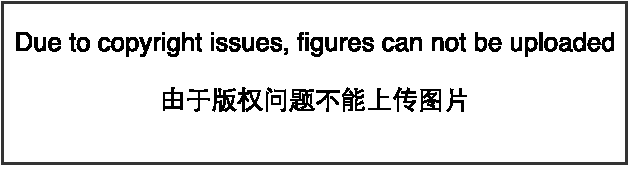
\includegraphics{figure.pdf}}
\else
\centerline{\includegraphics{Chapter5/figures/decision_tree}}
\fi
\caption{TODO}
\label{fig:chap5_decision_tree}
\end{figure}

正如我们已经看到的,最近邻预测和决策树都有很多的局限性。
尽管如此,在计算资源受限制时,它们都是很有用的学习算法。
通过思考复杂算法和$k$-最近邻或决策树之间的相似性和差异,我们可以建立对更复杂学习算法的直觉。

参考\cite{MurphyBook2012,bishop-book2006,Hastie2001}或其他\gls{ML}教科书了解更多的传统\gls{supervised_learning}算法。

\section{\glsentrytext{unsupervised_learning}算法}
\label{sec:unsupervised_learning_algorithms}
回顾第5.1.3节,无监督算法只处理“\gls{feature}”,不操作监督信号。
监督和无监督算法之间的区别没有规范,严格的定义,因为没有客观的判断来区分监督者提供的值是\gls{feature}还是\gls{target}。
通俗地说,\gls{unsupervised_learning}是指从不需要人为注释\gls{example:chap5}的分布中抽取信息的大多数尝试。
该术语通常与密度估计相关,学习从分布中采样,学习从分布中降噪,需要数据分布的流形,或是将数据中相关的\gls{example:chap5}聚类。

一个经典的\gls{unsupervised_learning}任务是找到数据的“最佳”表示。
“最佳”可以是不同的表示,但是一般来说,是指该表示在比本身表示的信息更简单或更易访问而受到一些惩罚或限制的情况下,尽可能保存关于$\Vx$更多的信息。 

% -- 142 --

有很多方式定义较简单的表示。最常见的三种包括低维表示,稀疏表示,独立表示。
低维表示尝试将$\Vx$中的信息尽可能压缩在一个较小的表示中。
稀疏表示将\gls{dataset}嵌入到输入项大多数为零的表示中\citep{Barlow89,Olshausen+Field-1996,Hinton+Ghahramani-97}。
稀疏表示通常用于需要增加表示维数的情况,使得大部分为零的表示不会丢失很多信息。
这会使得表示的整体结构倾向于将数据分布在表示空间的坐标轴上。
独立表示试图解开数据分布中变动的来源,使得表示的维度是统计独立的。

当然这三个标准并非相互排斥的。
低维表示通常会产生比原始的高维数据具有较少或较弱依赖关系的元素。
这是因为减少表示大小的一种方式是找到并消除冗余。
识别并去除更多的冗余使得降维算法在丢失更少信息的同时显现更大的压缩。

表示的概念是\gls{DL}核心主题之一,因此也是本书的核心主题之一。
本节会介绍表示学习算法中的一些简单实例。
总的来说,这些实例算法会说明如何实施上面的三个标准。
剩余的大部分章节会介绍其他表示学习算法以不同方式处理这三个标准或是介绍其他标准。

\subsection{\glssymbol{PCA}}
\label{sec:principal_components_analysis_chap5}
在第2.12节中,我们看到\glssymbol{PCA}算法提供了一种压缩数据的方式。
我们也可以将\glssymbol{PCA}视为学习数据表示的\gls{unsupervised_learning}算法。
这种表示基于上述简单表示的两个标准。
\glssymbol{PCA}学习一种比原始输入低维的表示。
它也学习了一种元素之间彼此没有线性相关的表示。
这是学习表示中元素统计独立标准的第一步。
要实现完全独立性,表示学习算法必须也去掉变量间的非线性关系。

% -- 143 --

如图\ref{fig:chap5_pca}所示,\glssymbol{PCA}将输入$\Vx$投影表示成$\Vz$,学习数据的正交,线性变换。
在第2.12节中,我们看到了如何学习重建原始数据的最佳一维表示(就\gls{mean_squared_error}而言),这种表示其实对应着数据的第一个主要成分。
因此,我们可以用\glssymbol{PCA}作为保留数据尽可能多信息的降维方法(再次是就最小重构误差平方而言)。
在下文中,我们将研究\glssymbol{PCA}表示如何使原始数据表示$\MX$去相关的.

\begin{figure}[!htb]
\ifOpenSource
\centerline{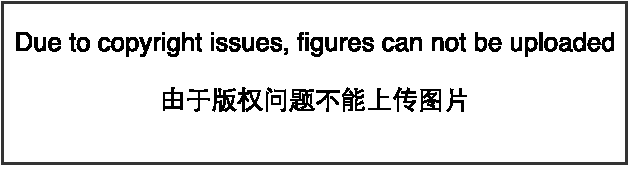
\includegraphics{figure.pdf}}
\else
\centerline{\includegraphics{Chapter5/figures/pca_color}}
\fi
\caption{TODO}
\label{fig:chap5_pca}
\end{figure}

假设有一个$m\times n$的\gls{design_matrix}$\MX$,数据的均值为零,$\SetE[\Vx] = 0$。
若非如此,通过预处理步骤所有\gls{example:chap5}减去均值,数据可以很容易地中心化。

$\MX$对应的无偏样本协方差矩阵给定如下
\begin{equation}
    \text{Var}[\Vx] = \frac{1}{m-1} \MX^\Tsp \MX .
\end{equation}
\glssymbol{PCA}会找到一个$\text{Var}[\Vz]$是对角矩阵的表示(通过线性变换)$\Vz=\Vx^\Tsp\MW$。

在第2.12节,我们看到\gls{design_matrix}$\MX$的主成分由$\MX^\Tsp\MX$的\gls{feature}向量给定。
从这个角度,我们有
\begin{equation}
    \MX^\Tsp\MX = \MW \VLambda \MW^\Tsp .
\end{equation}
本节中,我们会探索主成分分析的另一种推导。
主成分也可以通过奇异值分解得到。
具体地,它们是$\MX$的右奇异向量。
为了说明这点,假设$\MW$是奇异值分解$\MX = \MU\VSigma\Vw$的右奇异向量。
以$\MW$作为特征向量基,我们可以得到原来的特征向量方程:
\begin{equation}
    \MX^\Tsp\MX = \left( \MU\VSigma \MW \right)^\Tsp \MU\VSigma \MW = 
    \MW \VSigma^2 \MW^\Tsp .
\end{equation}

% -- 144 --

\glssymbol{SVD}有助于说明\glssymbol{PCA}后的$\text{Var}[\Vz]$是对角的。
使用$\MX$的\glssymbol{SVD}分解,$\MX$的方差可以表示为
\begin{align}
    \text{Var}[\Vx] &= \frac{1}{m-1} \MX^\Tsp\MX \\
    &= \frac{1}{m-1} \left( \MU\VSigma \MW \right)^\Tsp \MU\VSigma \MW \\
    &= \frac{1}{m-1} \MW \VSigma^\Tsp \MU^\Tsp \MU\VSigma \MW \\
    &= \frac{1}{m-1} \MW \VSigma^2 \MW ,
\end{align}
其中,我们使用$\MU^\Tsp\MU = \MI$,因为根据奇异值的定义矩阵$\MU$是正交的。
这表明,如果我们取$\MZ=\Vx\MW$,那么我们可以确保$\Vz$的协方差满足对角的要求:
\begin{align}
    \text{Var}[\Vz] &= \frac{1}{m-1} \MZ^\Tsp\MZ \\
    &= \frac{1}{m-1} \MW^\Tsp \MX^\Tsp \MX^\Tsp \MW \\
    &= \frac{1}{m-1} \MW^\Tsp\MW \VSigma^2 \MW^\Tsp\MW \\
    &= \frac{1}{m-1} \VSigma^2 ,
\end{align}
其中,再次使用\glssymbol{SVD}的定义有$\MW^\Tsp\MW = \MI$。

以上分析指明当我们通过线性变换$\MW$将数据$\Vx$投影到$\Vz$时,得到的数据表示的协方差矩阵是对角的($\VSigma^2$),即说明$\Vz$中的元素是彼此无关的。

\glssymbol{PCA}这种将数据变换为元素之间彼此不相关表示的能力是\glssymbol{PCA}的一个重要性质。
它是\emph{消除数据中未知变动因素}的简单表示实例。
在\glssymbol{PCA}中,这个消除是通过寻找输入空间的一个旋转(由$\MW$确定),
使得方差的主坐标和$\Vz$相关的新表示空间的基对齐。

% -- 145 --

虽然相关性是数据元素间依赖关系的一个重要范畴,但我们对于能够消除\gls{feature}依赖更复杂形式的表示学习也很有兴趣。
对此,我们需要比简单线性变换能做到更多的工具。

\subsection{$k$-均值聚类}
\label{sec:k_means_clustering}
另外一个简单的表示学习算法是$k$-均值聚类。
$k$-均值聚类算法将训练集分成$k$个靠近彼此的不同\gls{example:chap5}聚类。
因此我们可以认为该算法提供了$k$-维的独热码向量$\Vh$以表示输入$\Vx$。
当$\Vx$属于聚类$i$时,有$h_i=1$,$\Vh$的其他项为零。

$k$-均值聚类提供的独热码也是一种稀疏表示,因为每个输入的对应表示大部分元素为零。
之后,我们会介绍能够学习更灵活的稀疏表示的一些其他算法(表示中不只一个非零项)。
独热码是稀疏表示的一个极端实例,丢失了很多分布式表示的优点。
独热码仍然有一些统计优点(自然地传达了相同聚类中的\gls{example:chap5}彼此相似的观点),
也具有计算上的优势,因为整个表示可以用一个单独的整数表示。

$k$-均值聚类初始化$k$个不同的中心点$\{\Vmu^{(1)},\dots,\Vmu^{(k)}\}$,然后迭代交换两个不同的步骤直到收敛。
步骤一,每个训练\gls{example:chap5}分配到最近的中心点$\Vmu^{(i)}$所代表的聚类$i$。
步骤二,每一个中心点$\Vmu^{(i)}$更新为聚类$i$中所有训练\gls{example:chap5}$\Vx^{(j)}$的均值。

关于聚类的一个问题是聚类问题本身是病态的。
这是说没有单一的标准去衡量聚类的数据对应真实世界有多好。
我们可以衡量聚类的性质,例如每个聚类的元素到该类中心点的平均欧几里得距离。
这使我们可以判断能够多好地从聚类分配中重建训练数据。
然而我们不知道聚类的性质多好地对应于真实世界的性质。
此外,可能有许多不同的聚类都能很好地对应到现实世界的某些属性。
我们可能希望找到和一个\gls{feature}相关的聚类,但是得到了一个和任务无关的不同的,同样是合理的聚类。
例如,假设我们在包含红色卡车图片,红色汽车图片,灰色卡车图片和灰色汽车图片的\gls{dataset}上运行两个聚类算法。
如果每个聚类算法聚两类,那么可能一个算法将汽车和卡车各聚一类,另一个根据红色和灰色各聚一类。
假设我们还运行了第三个聚类算法,用来决定类别的数目。
这有可能聚成了四类,红色卡车,红色汽车,灰色卡车和灰色汽车。
现在这个新的聚类至少抓住了属性的信息,但是损失掉了相似性信息。
红色汽车和灰色汽车在不同的类中,正如红色汽车和灰色卡车也在不同的类中。
该聚类算法没有告诉我们灰色汽车比灰色卡车和红色汽车更相似。
我们只知道它们是不同的。

% -- 146 --

这些问题说明了一些我们可能更偏好于分布式表示(相对于独热码表示而言)的原因。
分布式表示可以对每个车辆赋予两个属性----一个表示它颜色,一个表示它是汽车还是卡车。
目前仍然不清楚什么是最优的分布式表示(学习算法如何知道我们关心的两个属性是颜色和是否汽车或卡车,而不是制造商和车龄?),
但是多个属性减少了算法去猜我们关心哪一个属性的负担,允许我们通过比较很多属性而非测试一个单一属性来细粒度地衡量相似性。

\section{\glsentrytext{SGD}}
\label{sec:stochastic_gradient_descent_chap5}
几乎所有的\gls{DL}算法都用到了一个非常重要的算法:\firstall{SGD}。
\gls{SGD}是第4.3节介绍的\gls{GD}算法的一个扩展。

\gls{ML}中的一个循环问题是大的\gls{dataset}是好的泛化所必要的,但大的训练集的计算代价也更大。

% -- 147 --

\gls{ML}算法中的损失函数通常可以分解成每个\gls{example:chap5}损失函数的总和。
例如,训练数据的负条件对数似然可以写成
\begin{equation}
    J(\Vtheta) = \SetE_{\Vx,y \sim \hat{p}_{\text{data}}}
    L(\Vx, y, \Vtheta) = 
    \frac{1}{m} \sum_{i=1}^m  L(\Vx^{(i)}, y^{(i)}, \Vtheta) ,
\end{equation}
其中$L$是每个\gls{example:chap5}的损失函数$L(\Vx, y, \Vtheta) = -\log p(y|\Vx;\Vtheta)$。

对于这些相加的损失函数,\gls{GD}需要计算
\begin{equation}
    \nabla_{\Vtheta} J(\Vtheta)
    = \frac{1}{m} \sum_{i=1}^m  
    \nabla_{\Vtheta} L(\Vx^{(i)}, y^{(i)}, \Vtheta) .
\end{equation}
这个运算的计算代价是$O(m)$。
随着训练集规模增长为数十亿的\gls{example:chap5},计算一步梯度也会消耗相当长的时间。

\gls{SGD}的核心是,梯度是期望。
期望可使用小规模的样本近似估计。
具体而言,在算法的每一步,我们从训练集中均匀抽出一\firstgls{minibatch}\gls{example:chap5}$\SetB=\{\Vx^{(1)},\dots,\Vx^{(m')}\}$。
\gls{minibatch}的数目$m'$通常是一个相对较小的数,从一到几百。
重要的是,当训练集大小$m'$增长时,$m$通常是固定的。
我们可能在拟合几十亿的\gls{example:chap5}时,每次更新计算只用到几百个\gls{example:chap5}。

梯度的估计可以表示成
\begin{equation}
    \Vg = \frac{1}{m'} \nabla_{\Vtheta} \sum_{i=1}^{m'}
    L(\Vx^{(i)}, y^{(i)}, \Vtheta)
\end{equation}
使用来自\gls{minibatch}$\SetB$的\gls{example:chap5}。
然后,\gls{SGD}算法使用如下的\gls{GD}估计:
\begin{equation}
    \Vtheta \leftarrow \Vtheta - \epsilon \Vg,
\end{equation}
其中,$\epsilon$是学习速率。

\gls{GD}往往被视为慢的或不可靠的。
以前,将\gls{GD}应用到非凸优化问题被视为鲁莽的或无原则的。
现在,我们知道\gls{GD}用于训练第二部分中工作效果很好。
优化算法可能不能保证在合理的时间内达到一个局部最小值,但它通常能足够快地找到损失函数的一个可以用的非常低的值。 

% -- 148 --

\gls{SGD}在\gls{DL}之外有很多重要的应用。
它是在大规模数据上训练大型线性模型的主要方法。
对于固定大小的模型,每一步\gls{SGD}更新的计算量不取决于训练集的大小$m$。
在实践中,当训练集大小增长时,我们通常会使用一个更大的模型,但这并非强制的。
达到收敛所需的更新次数通常会随训练集规模增大而增加。
然而,当$m$趋向于无限时,该模型最终会在\gls{SGD}抽样训练集上的每个\gls{example:chap5}前
收敛到可能的最优测试误差。
继续增加$m$不会延长达到模型可能的最优测试误差的时间。
从这点来看,我们可以认为用\gls{SGD}训练模型的渐近代价是关于$m$的函数的$O(1)$级别。

在\gls{DL}之前,学习非线性模型的主要方法是结合核技巧的线性模型。
很多核学习算法需要构建一个$m\times m$的矩阵$G_{i,j}=k(\Vx^{(i)}, \Vx^{(j)})$。
构建这个矩阵的计算量是$O(m^2)$。
当\gls{dataset}是几十亿个\gls{example:chap5}时,这个计算量是不能接受的。
在学术界,\gls{DL}从2006年开始收到关注的原因是,在数以万计\gls{example:chap5}的中等规模\gls{dataset}上,\gls{DL}在新\gls{example:chap5}上比当时很多热门算法泛化得更好。
不久后,\gls{DL}在工业界受到了更多的关注,因为其提供了一种可扩展的方式训练大\gls{dataset}上的非线性模型。

\gls{SGD}及其很多强化方法将会在第\ref{chap:optimization_for_training_deep_models}章继续探讨。

\section{构建\glsentrytext{ML}算法}
\label{sec:building_a_machine_learning_algorithm}
几乎所有的深学习算法可以被描述为一个相当简单的配方:特定的\gls{dataset},损失函数,优化过程和模型。

例如,\gls{linear_regression}算法的组成成分有$\MX$和$\Vy$构成的\gls{dataset},损失函数
\begin{equation}
    J(\Vw, b) = -\SetE_{\Vx,y\sim\hat{p}_{\text{data}}}
    \log p_{\text{model}} (y | \Vx) ,
\end{equation}
模型是$p_{\text{model}} (y | \Vx) \mathcal{N}(y; \Vx^\Tsp \Vw + b, 1)$,
在大多数情况下,优化算法可以定义为求解损失函数梯度为零的标准方程。

意识到我们可以替换独立于其他成分的大多数成分,因此我们能得到很多不同的算法。

% -- 149 --

损失函数通常包括使学习过程执行统计估计的至少一项。
最常见的损失函数是负对数似然,最小化损失函数导致的\gls{maximum_likelihood_estimation}。

损失函数也可能含有附加项,如\gls{regularizer}。
例如,我们可以将权重衰减加到\gls{linear_regression}的损失函数中
\begin{equation}
    J(\Vw, b) = \lambda \norm{\Vw}_2^2 - \SetE_{\Vx,y\sim p_{\text{data}}}
    \log p_{\text{model}} (y | \Vx) .
\end{equation}
该优化仍然有闭解。

如果我们将该模型变成非线性的,那么大多数损失函数不再有优化闭解。
这就要求我们选择一个迭代数值优化过程,如\gls{GD}等。

组合模型,损失函数和优化算法来构建学习算法的配方同时适用于\gls{supervised_learning}和\gls{unsupervised_learning}。
\gls{linear_regression}实例说明了如何适用于\gls{supervised_learning}的。
\gls{unsupervised_learning}时,我们需要定义一个只包含$\MX$的\gls{dataset},一个合适的无监督损失函数和一个模型。
例如,通过指定如下损失函数可以得到\glssymbol{PCA}的第一个主向量
\begin{equation}
    J(\Vw) = \SetE_{\Vx \sim p_{\text{data}}} \norm{\Vx - r(\Vx; \Vw)}_2^2
\end{equation}
模型定义为重建函数$r(\Vx) = \Vw^\Tsp\Vx \Vw$,并且$\Vw$有范数为$1$的限制。

在某些情况下,由于计算原因,我们不能实际计算损失函数。
在这种情况下,只要我们有近似其梯度的方法,那么我们仍然可以使用迭代数值优化近似最小化\gls{target}。

大多数学习算法都用到了上述配方,尽管有时候不显然。
如果一个\gls{ML}算法看上去特别独特或是手动设计的,那么通常使用特殊的优化方法进行求解。
有些模型,如决策树或$k$-均值,需要特殊的优化,因为它们的损失函数有平坦的区域,
使其不适合通过基于梯度的优化去最小化。
认识到大部分\gls{ML}算法可以使用上述配方描述,有助于将不同算法视为出于相同原因解决相关问题的一类方法,而不是一长串各个不同的算法。

% -- 150 --

\section{推动\glsentrytext{DL}的挑战}
\label{sec:challenges_motivating_deep_learning}
本章描述的简单\gls{ML}算法在很多不同的重要问题上都效果良好。
但是他们不能成功解决人工智能中的核心问题,如语音识别或者实物识别。

\gls{DL}发展动机的一部分原因是传统学习算法在这类人工智能问题上泛化能力不行。

本节介绍为何处理高维数据时在新\gls{example:chap5}上泛化变得特别困难,以及为何传统\gls{ML}中实现泛化的机制不适合学习高维空间中复杂的函数。
这些空间经常涉及巨大的计算代价。
\gls{DL}旨在克服这些,以及其他困难。

\subsection{\glsentrytext{curse_of_dimensionality}}
\label{sec:the_curse_of_dimensionality}
当数据的维数很高时,很多\gls{ML}问题变得相当困难。
这种现象被称为\firstgls{curse_of_dimensionality}(curse of dimensionality)。
特别值得注意的是,一组变量的不同可能配置数量随着变量数目的增加而指数级增长。

维数灾难发生在计算机科学的许多地方,在\gls{ML}中尤其如此。

由\gls{curse_of_dimensionality}带来的一个挑战是统计挑战。
如图\ref{fig:chap5_curse}所示,统计挑战产生于$\Vx$的可能配置数目远大于训练\gls{example:chap5}的数目。
为了充分理解这个问题,我们假设输入空间如图所示被分成网格。
低维时我们可以用由数据占据的少量网格去描述这个空间。
泛化到新数据点时,通过检测和新输入在相同网格中的训练\gls{example:chap5},我们可以判断如何处理新数据点。
例如,如果要估计某点$\Vx$处的概率密度,我们可以返回$\Vx$处单位体积内训练\gls{example:chap5}的数目除以训练\gls{example:chap5}的总数。
如果我们希望对一个\gls{example:chap5}进行分类,我们可以返回相同网格中训练\gls{example:chap5}最多的类别。
如果我们是做回归分析,我们可以平均该网格中\gls{example:chap5}对应的的\gls{target}值。
但是,如果该网格中没有\gls{example:chap5},该怎么办呢?
因为在高维空间中参数配置数目远大于\gls{example:chap5}数目,大部分配置没有相关的\gls{example:chap5}。
我们如何能在这些新配置中找到一些有意义的东西?
许多传统\gls{ML}算法简单地假设在一个新点的输出应大致和最接近的训练点的输出相同。


\begin{figure}[!htb]
\ifOpenSource
\centerline{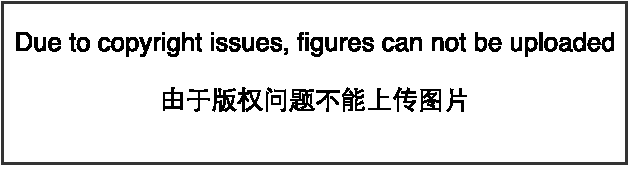
\includegraphics{figure.pdf}}
\else
\begin{tabular}{ccc}
    \includegraphics[width=0.3\textwidth]{Chapter5/figures/curse_1d_color} & \includegraphics[width=0.3\textwidth]{Chapter5/figures/curse_2d_color} & \includegraphics[width=0.3\textwidth]{Chapter5/figures/curse_3d_color}
\end{tabular}
\fi
\caption{TODO}
\label{fig:chap5_curse}
\end{figure}

% -- 151 --

\subsection{局部不变性和平滑\glsentrytext{regularization}}
\label{sec:local_constancy_and_smoothness_regularization}
为了更好地泛化,\gls{ML}算法需要由先验信念引导应该学习什么类型的函数。
此前,我们已经看到过由模型参数上的概率分布形成的先验。
更非正式地,我们也可以探讨先验信念如何直接影响\emph{函数}本身,间接影响参数,作为参数与函数之间关系的结果。 
此外,我们也可以非正式地探讨隐式表示的先验。
某些算法有偏地选择某类函数,即使这类有偏可能不能表示成(或者可能表示成)我们对不同函数偏好程度的概率分布。

% -- 152 --

其中最广泛使用的隐式“先验”是\firstgls{smoothness_prior},或\firstgls{local_constancy_prior}。
这个先验表明我们学习的函数不应在小区域内发生很大的变化。

许多简单算法完全依赖于此先验达到良好的泛化,其结果是不能推广去解决\gls{AI}级别任务中的统计挑战。
本书中,我们将介绍\gls{DL}如何引入额外的(显示的和隐式的)先验去降低复杂任务中的泛化误差。
这里,我们解释为什么单是平滑先验不足以应对这类任务。

有许多不同的方法来隐式地或显式地表示学习函数应该是光滑或局部不变的先验。
所有这些不同的方法都旨在鼓励学习过程能够学习出函数$f^*$满足条件
\begin{equation}
    f^*(\Vx) \approx f^*(\Vx + \epsilon)
\end{equation}
对于大多数设置$\Vx$和小变动$\epsilon$都成立。
换言之,如果我们在输入$\Vx$处效果良好(例如,$\Vx$是一个有\gls{label}的训练\gls{example:chap5}),那么在$\Vx$的邻域上效果也良好。
如果在有些邻域中我们有几个好答案,那么我们可以组合它们(通过某种形式的平均或插值法)以产生一个尽可能和大多数输入一致的答案。

局部不变方法的一个极端例子是$k$-最近邻型的学习算法。
预测在所有点$\Vx$都有相同的$k$个训练集中最近邻点的区域上是不变的。
当$k=1$时,不同区域的数目不可能比训练\gls{example:chap5}还多。

虽然$k$近邻算法拷贝了附近训练\gls{example:chap5}的输出,大部分核机器也是在和附近训练\gls{example:chap5}相关的训练集输出上插值。
一类重要的核函数是\firstgls{local_kernel},其核函数$k(\Vu,\Vv)$在$\Vu=\Vv$时很大,
当$\Vu$和$\Vv$距离拉大时而减小。
局部核可以看作是执行模版匹配的相似函数,衡量测试\gls{example:chap5}$\Vx$和每个训练\gls{example:chap5}$\Vx{(i)}$有多么相似。
大部分\gls{DL}的现代动机源自研究局部模版匹配的局限性,以及\gls{DL}如何克服这些局限性\citep{NIPS2005_424}。

决策树也有平滑学习的局限性,因为它将输入空间分成和叶节点一样多的区间,并在每个区间使用单独的参数(或者有些决策树的拓展有多个参数)。
如果\gls{target}函数需要至少$n$个叶节点的树去精确表示,那么至少需要$n$个训练\gls{example:chap5}去拟合。
需要几倍于$n$的\gls{example:chap5}去达到预测输出上的某种统计置信度。

% -- 153 --

总的来说,区分输入空间中$O(k)$个区间,所有的这些方法需要$O(k)$个\gls{example:chap5}。
通常会有$O(k)$个参数,$O(1)$参数对应于$O(k)$区间之一。
最近邻中,每个训练\gls{example:chap5}至多用于定义一个区间,如图5.10所示。

有没有什么方法能表示区间数目比训练\gls{example:chap5}数目还多的复杂函数?
显然,只是假设函数的平滑性不能做到这点。
例如,想象\gls{target}函数是一种棋盘。
棋盘包含许多变化,但只有一个简单的结构。
想象一下,如果训练\gls{example:chap5}数目远小于棋盘上的黑白方块数目,那么会发生什么。
基于局部泛化和平滑性或局部不变性先验,如果新点和某个训练\gls{example:chap5}位于相同的棋盘方块中,那么我们能够保证正确预测新点的颜色。
但如果新点位于棋盘中不包含训练\gls{example:chap5}的方块中,没有保证预测能够正确。
单单是这个先验,一个\gls{example:chap5}只能告诉我们它所在的方块的颜色。
获得在整个棋盘颜色的唯一方法是其上的每个方块至少要有一个\gls{example:chap5}。

% -- 154 --

只要在要学习的真实函数的峰值和谷值处有足够多的\gls{example:chap5},那么平滑性假设和相关的无参数学习算法的效果都非常好。
当要学习的函数足够平滑,并且只在少数几维变动,这一般是对的。
在高维空间中,即使是非常平滑的函数,也会在不同维度上有不同的平滑变动程度。
如果函数在不同的区间中表现不一样,那么就非常难用一组训练\gls{example:chap5}去刻画函数。
如果函数是复杂的(我们希望区分多于训练\gls{example:chap5}数目的大量区间),有希望很好地泛化么?

回答这些问题----是否可以有效地表示复杂的函数,以及所估计的函数是否可以良好地泛化到新的输入----有。
关键观点是,只要我们在区间相关性上引入额外的数据生成分布上的假设,那么$O(k)$个\gls{example:chap5}是足以描述多如$O(2^k)$的大量区间。
这样,我们真的能做到非局部地泛化\citep{Bengio+Monperrus-2005,NIPS2005_539}。
许多不同的\gls{DL}算法提出隐式或显式的适用于大范围人工智能问题的合理假设, 使其可以利用这些优势。

其他的一些\gls{ML}方法往往会提出更强的,针对特定问题的假设。
例如,假设\gls{target}函数是周期性的,我们很容易解决棋盘问题。
通常,我们在神经网络中不包含这些很强的,针对特定任务的假设,从而使神经网络可以泛化到更广泛的各种结构中。
人工智能任务的结构非常复杂,很难限制到简单的,人工手动制定的性质,如周期性,因此我们希望学习算法具有更通用的假设。
\gls{DL}中的核心思想是我们假设数据由\emph{因素或特征组合},也可能是由层次结构中多个层级产生。
许多其他类似的通用假设进一步提高了\gls{DL}算法。
这些很温和的假设允许\gls{example:chap5}数目和区间数目之间的关系有指数增益。
这类指数增益将在第6.4.1节,第15.4节和第15.5节中被更详尽地介绍。
深度分布式表示带来的指数增益有效应对了\gls{curse_of_dimensionality}引来的挑战。

% -- 155 --

\subsection{\glsentrytext{manifold_learning}}
\label{sec:manifold_learning}
在\gls{ML}很多想法背后的一个重要概念是\gls{manifold}。

\firstgls{manifold}指连接在一起的区域。
数学上,它是指一组点,且每个点都有其邻域。
给定一个任意的点,其流形局部看起来像是欧几里得空间。
日常生活中,我们将世界视为2-D平面,但实际上它是3-D的球形\gls{manifold}。

每个点周围邻域的定义暗示着存在变换能够从一个位置移动到其邻域位置。
例如在地球表面这个流形中,我们可以朝东南西北走。

尽管术语“流形”有正式的数学定义,\gls{ML}倾向于更松散地定义一组点,使其只需要考虑少数嵌入在高维空间中的自由度或维数就能很好地近似。
每一维都对应着局部的变动方向。
如图\ref{sec:challenges_motivating_deep_learning}所示,训练数据位于二维空间中的一维流形中。
在\gls{ML}中,我们允许流形的维数从一个点到另一个点有所变化。
这经常发生于流形和自身相交的情况。
例如,数字“8”形状的流形在大多数位置只有一维,但在中心的相交处有两维。

如果我们希望\gls{ML}算法学习$\SetR^n$上的所有感兴趣的函数时,很多\gls{ML}问题
看上去都是不可解的。
\firstgls{manifold_learning}算法,通过假设$\SetR^n$中大部分区域无效的输入,感兴趣的输入只分布在包含少量点的子集构成的一组流形中,而学习函数中感兴趣输出的变动只位于流形中的方向,或者感兴趣的变动只发生在我们从一个流形移动到另一个流形时,克服这个障碍。
流形学习是在连续数值数据和\gls{unsupervised_learning}的设定下被引入的,尽管这个概率集中的想法也能够泛化到离散数据和\gls{supervised_learning}的设定下:关键假设仍然是概率质量高度集中。

% -- 156 --

数据位于低维流形的假设并不总是对的或者有用的。
我们认为在人工智能的一些场景中,如涉及到处理图像,声音或者文本,流形假设至少是
近似对的。
这个假设的支持证据包含两类观察结果。

第一个支持\firstgls{manifold_hypothesis}的观察是现实生活中的图像,文本,声音的
概率分布都是高度集中的。
均匀的噪音从来没有和这类领域的结构化输入相似过。
图\ref{fig:chap5_noise}显示均匀采样的点看上去像是没有信号时模拟电视上的静态模式。
同样,如果您均匀地随机抽取字母来生成文件,能有多大的概率会得到一个有意义的英语文档?
几乎是零。因为大部分字母长序列不对应着自然语言序列:
自然语言序列的分布只占了字母序列的总空间里非常小的体积。

\begin{figure}[!htb]
\ifOpenSource
\centerline{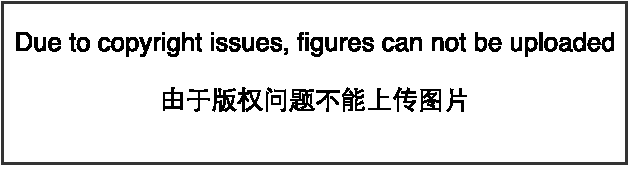
\includegraphics{figure.pdf}}
\else
\centerline{\includegraphics[width=0.7\textwidth]{Chapter5/figures/noise}}
\fi
\caption{TODO}
\label{fig:chap5_noise}
\end{figure}

当然,集中的概率分布不足以说明数据位于一个相当小的流形中。
我们还必须确定,我们遇到的\gls{example:chap5}和其他\gls{example:chap5}相互连接,每个\gls{example:chap5}被其他高度相似的\gls{example:chap5}包围,可以通过应用变换来遍历该流形。
支持流形假设的第二个论点是,我们至少能够非正式地想象这些邻域和变换。
在图像中,我们当然会认为有很多可能的变换允许我们描绘出图片空间的流形:
我们可以逐渐变暗或变亮光泽,逐步移动或旋转图中对象,逐渐改变对象表面的颜色,等等。
在大多数应用中很有可能会涉及多个流形。
例如,人脸图像的\gls{manifold}不太可能连接到猫脸图像的\gls{manifold}。

% -- 157 --

这些支持流形假设的思维试验传递了一些支持它的直观理由。
更严格的实验\citep{Cayton-2005,Narayanan+Mitter-NIPS2010,Scholkopf98-book,Roweis2000-lle-small,Tenenbaum2000-isomap,Brand2003,Belkin+Niyogi-nips2003,Donoho+Carrie-03,Weinberger04a}在\gls{AI}中感兴趣的一大类\gls{dataset}上支持了这个假设。

当数据位于低维流形中,使用流形中的坐标,而非$\SetR^n$中的坐标表示\gls{ML}中的数据更为自然。
日常生活中,我们可以认为道路是嵌入在三维空间的一维流形。
我们用1-D道路中的地址号码去明确地址,而非3-D空间中的坐标。
提取这些流形中的坐标是非常具有挑战性的,但是很有希望改进很多\gls{ML}算法。
这个一般性原则用于很多情况下。
图5.13展示了包含脸的\gls{dataset}的流形结构。
在本书的最后,我们会介绍一些学习这样的流形结构的必备方法。
在图20.6中,我们将看到\gls{ML}算法如何能成功地完成这个\gls{target}。

第一部分介绍了数学和\gls{ML}中的基本概念,这将用于本书其他章节中。
至此,您现在已经准备好了开始学习\gls{DL}。

% -- 159 --



